\documentclass[11pt,a4paper]{article}
\usepackage[utf8]{inputenc}
\usepackage[margin=1in]{geometry}
\setlength{\headheight}{14pt}
\usepackage{graphicx}
\usepackage{amsmath,amssymb}
\usepackage{booktabs}
\usepackage{array}
\usepackage{hyperref}
\usepackage{float}
\usepackage{caption}
\usepackage{subcaption}
\usepackage{fancyhdr}
\usepackage{titlesec}
\usepackage{xcolor}

% Custom Colors
\definecolor{primary}{RGB}{0, 51, 102}
\definecolor{secondary}{RGB}{70, 130, 180}

\hypersetup{
    colorlinks=true,
    linkcolor=primary,
    citecolor=primary,
    urlcolor=secondary
}

% Header and Footer setup
\pagestyle{fancy}
\fancyhf{}
\rhead{\textcolor{primary}{\textbf{EDC Laboratory --- Experiment 1}}}
\lhead{\textcolor{primary}{\textbf{EE25BTECH11056 \& EE25BTECH11049}}}
\rfoot{Page \thepage}

\titleformat{\section}{\large\bfseries\color{primary}}{\thesection.}{0.5em}{}
\titleformat{\subsection}{\normalfont\bfseries\color{secondary}}{\thesubsection}{0.5em}{}

\begin{document}

% Title Page / Header Block
\begin{center}
    {\LARGE \textbf{\color{primary} DEPARTMENT OF ELECTRICAL ENGINEERING}}\\[0.2cm]
    {\large \textbf{Electronic Devices \& Circuits Laboratory (EDC LAB)}}\\[0.5cm]
    \rule{\linewidth}{1pt}\\[0.4cm]
    {\Large \textbf{EXPERIMENT 1: V--I Characteristics of PN Junction \& Zener Diodes, and Study of Clipper \& Clamper Circuits}}\\[0.4cm]
    \rule{\linewidth}{1pt}\\[0.6cm]
    
    \begin{tabular}{ll}
        \textbf{Prepared By:} & Suraj.N (EE25BTECH11056) \\
                             & Sai Krishna Bakki (EE25BTECH11049) \\
        \textbf{Course:} & Electronic Devices \& Circuits Lab \\
        \textbf{Date:} & \today
    \end{tabular}
\end{center}

\vspace{0.5cm}

\section{Aim}
\begin{enumerate}
    \item To plot the forward- and reverse-bias $V$--$I$ characteristics of a PN junction diode and determine its cut-in voltage (\textbf{$V_\gamma$}), static forward resistance (\textbf{$R_{DC}$}), dynamic forward resistance (\textbf{$r_d$}), and reverse saturation current (\textbf{$I_s$}).
    \item To plot the forward- and reverse-bias $V$--$I$ characteristics of a Zener diode (1N4733A) and determine its Zener breakdown voltage (\textbf{$V_Z$}) and Zener resistance (\textbf{$R_Z$}).
    \item To design, simulate, and test positive, negative, and biased (two-level) diode clipper circuits and observe their clipping levels.
    \item To design, simulate, and test positive and negative diode clamper circuits and measure the resulting DC voltage shift.
\end{enumerate}

\section{Apparatus and Software Tools Required}
\begin{table}[H]
\centering
\caption{Equipment and Components Specifications}
\begin{tabular}{cllc}
\toprule
\textbf{S.No.} & \textbf{Component / Equipment} & \textbf{Specification} & \textbf{Quantity} \\
\midrule
1 & PN Junction Diode & 1N4007 / 1N4148 & 1 \\
2 & Zener Diode & 1N4733A ($V_Z = 5.1\text{ V}, 1\text{ W}$) & 1 \\
3 & Resistors & $1\text{ k}\Omega$, $10\text{ k}\Omega$, $100\text{ k}\Omega$ & As required \\
4 & Capacitor & $0.1\text{ }\mu\text{F}$ & 1 \\
5 & DC Voltage Sources & $0$--$30\text{ V}$ Variable, $+1\text{ V}$, $-1\text{ V}$ Reference & As required \\
6 & Function Generator / AC Source & $1\text{ kHz}$ Sine wave, $4\text{ V}_{pp}$ & 1 \\
7 & Simulation Software & LTspice & -- \\
8 & Digital Storage Oscilloscope (DSO) & Hardware measurement & 1 \\
\bottomrule
\end{tabular}
\end{table}

\newpage
\section{Part A: PN Junction Diode Characteristics}

\subsection{Theoretical Background}
A PN junction diode exhibits non-linear current-voltage characteristics described by the Shockley diode equation:
\begin{equation}
I = I_s \left( e^{\frac{V}{\eta V_T}} - 1 \right)
\end{equation}
where $I_s$ is the reverse saturation current, $V_T = \frac{k T}{q}$ is the thermal voltage ($\approx 26\text{ mV}$ at room temperature), and $\eta$ is the ideality factor.
\begin{itemize}
    \item \textbf{Forward Bias:} Below cut-in voltage (\textbf{$V_\gamma \approx 0.6\text{--}0.7\text{ V}$} for Silicon), current is negligible. Above \textbf{$V_\gamma$}, current increases exponentially.
    \item \textbf{Reverse Bias:} Barrier height increases, allowing only minute reverse saturation current \textbf{$I_s$} to flow until reverse breakdown occurs.
\end{itemize}

\subsection{Circuit Diagrams and Simulation Waveforms}

\subsubsection{PN Junction Diode -- Forward Bias}
\begin{figure}[H]
    \centering
    
\includegraphics[width=0.65\textwidth]{../DIODE_FORWARD/circuit.png}
    \caption{PN Junction Diode Forward Bias Circuit Schematic.}
    \label{fig:diode_fwd_circuit}
\end{figure}

\begin{figure}[H]
    \centering
    \begin{subfigure}[b]{0.42\textwidth}
        \centering
        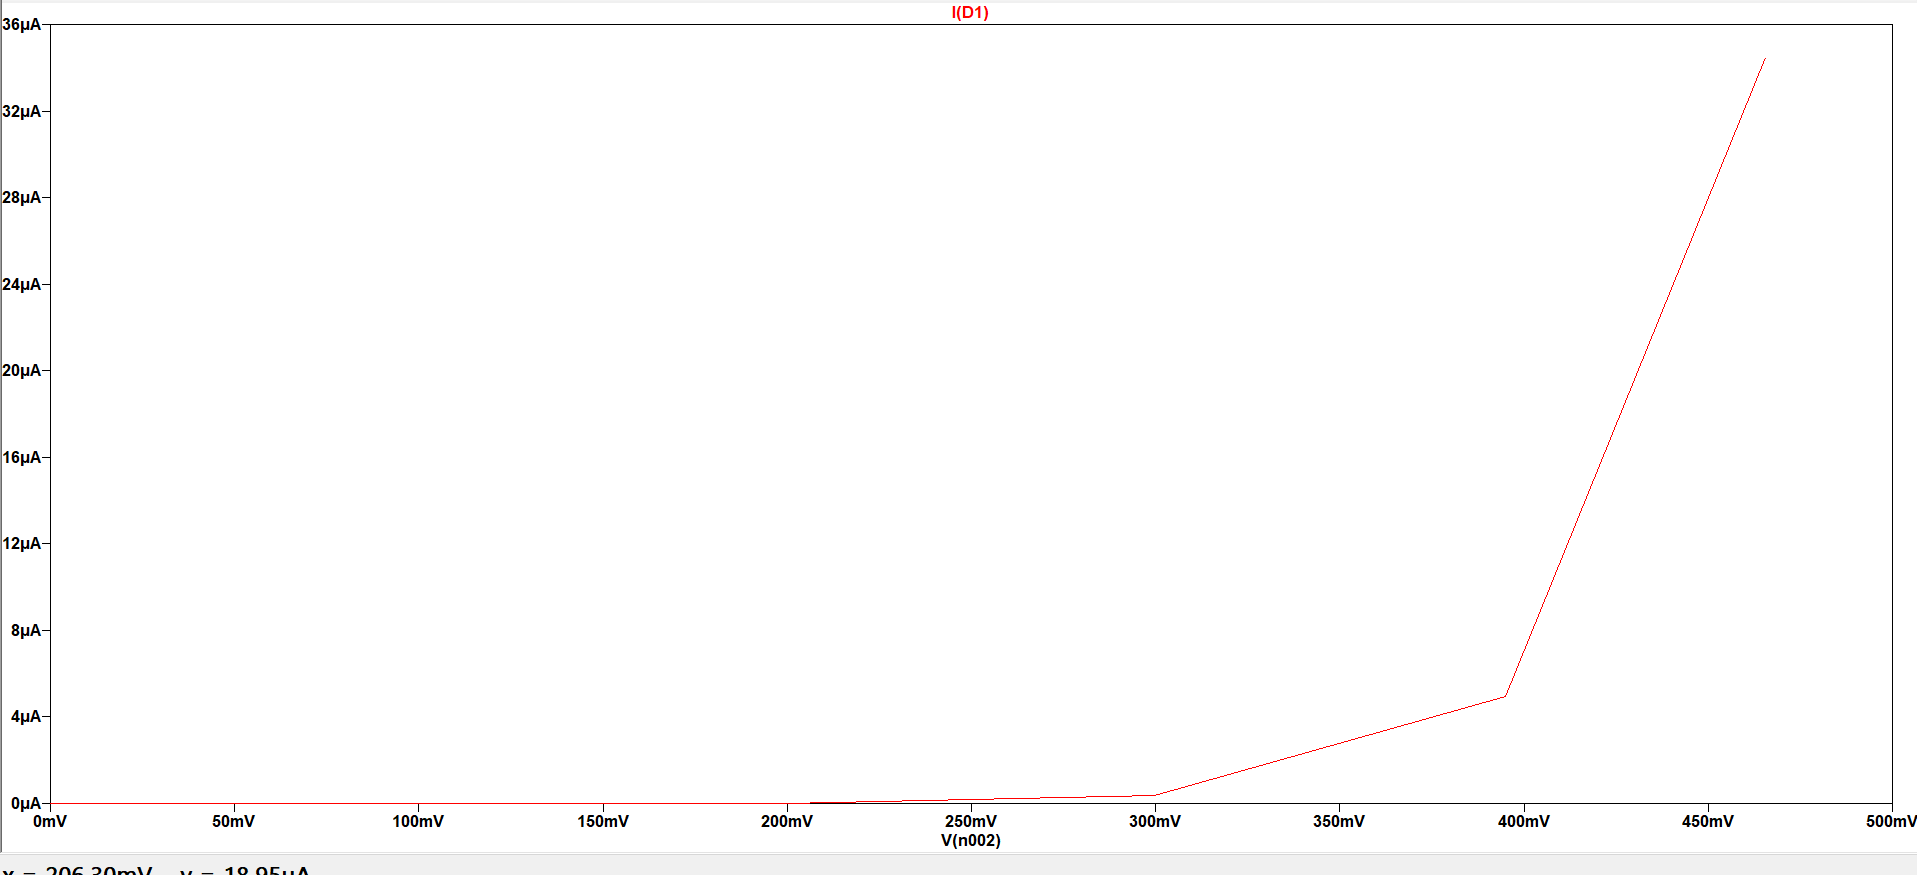
\includegraphics[width=\textwidth]{../DIODE_FORWARD/0-0.5v.png}
        \caption{Low Voltage Sweep ($0\text{ V}$ to $0.5\text{ V}$)}
    \end{subfigure}
    \hfill
    \begin{subfigure}[b]{0.42\textwidth}
        \centering
        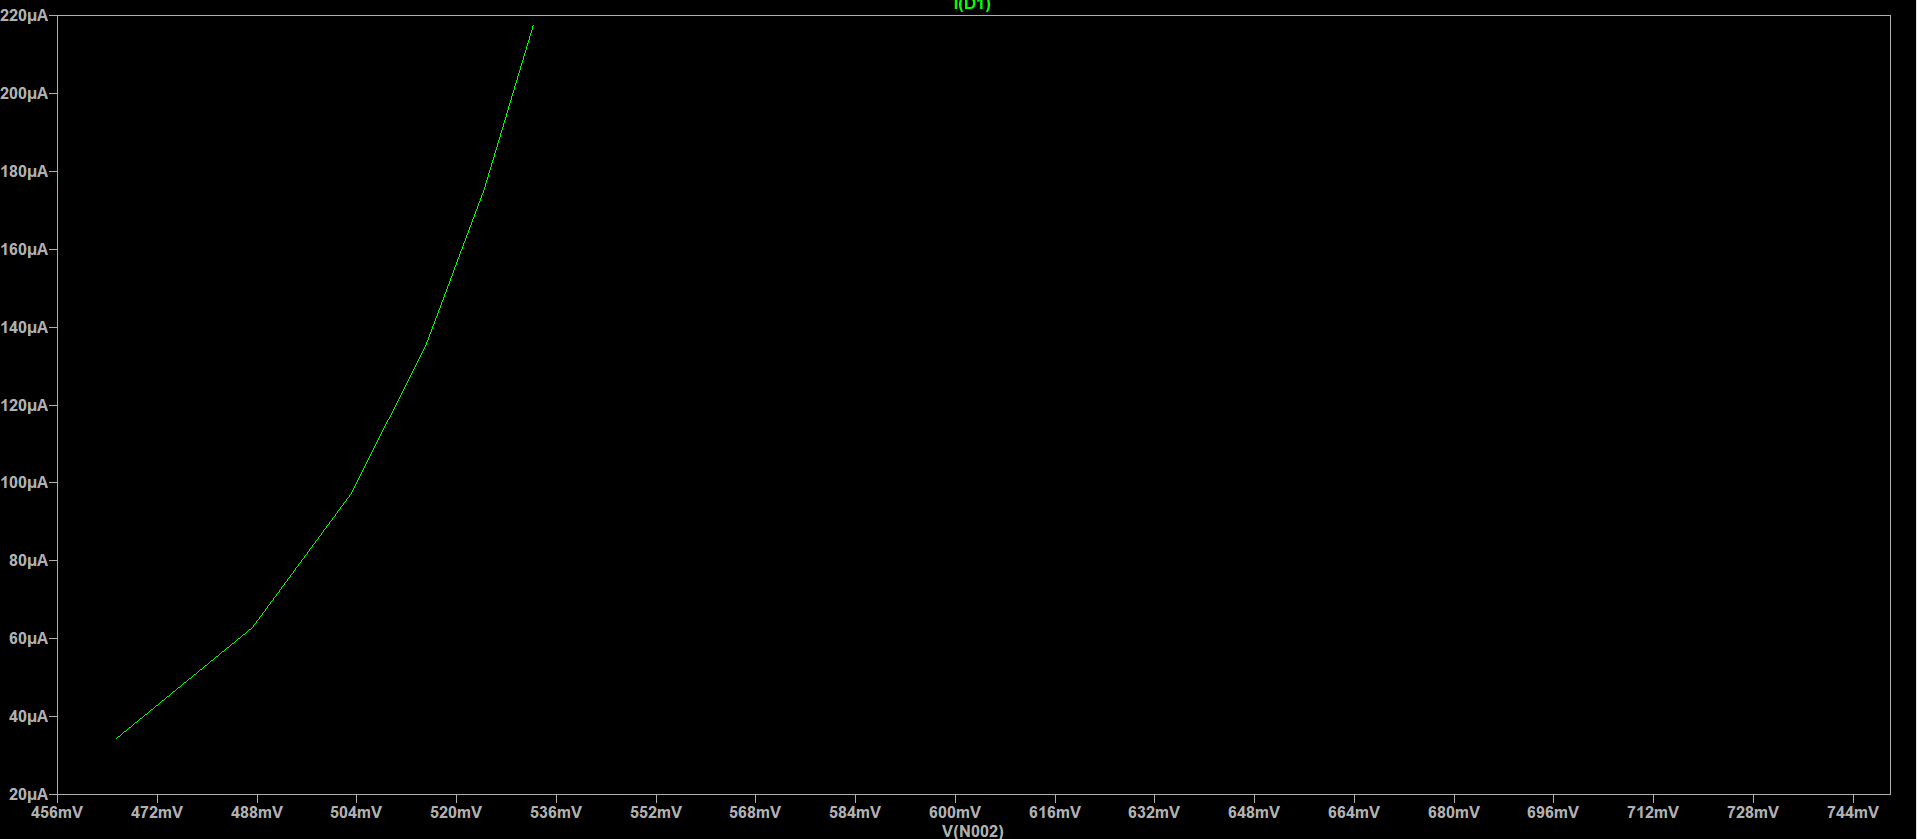
\includegraphics[width=\textwidth]{../DIODE_FORWARD/0.5-0.75v.png}
        \caption{Knee Region Sweep ($0.5\text{ V}$ to $0.75\text{ V}$)}
    \end{subfigure}
    \caption{PN Diode Forward $V$--$I$ Characteristics Simulation Plots.}
    \label{fig:diode_fwd_sim}
\end{figure}

\subsubsection{PN Junction Diode -- Reverse Bias}
\begin{figure}[H]
    \centering
    
\includegraphics[width=0.65\textwidth]{../DIODE_REVERSE/circuit.png}
    \caption{PN Junction Diode Reverse Bias Circuit Schematic.}
    \label{fig:diode_rev_circuit}
\end{figure}

\begin{figure}[H]
    \centering
    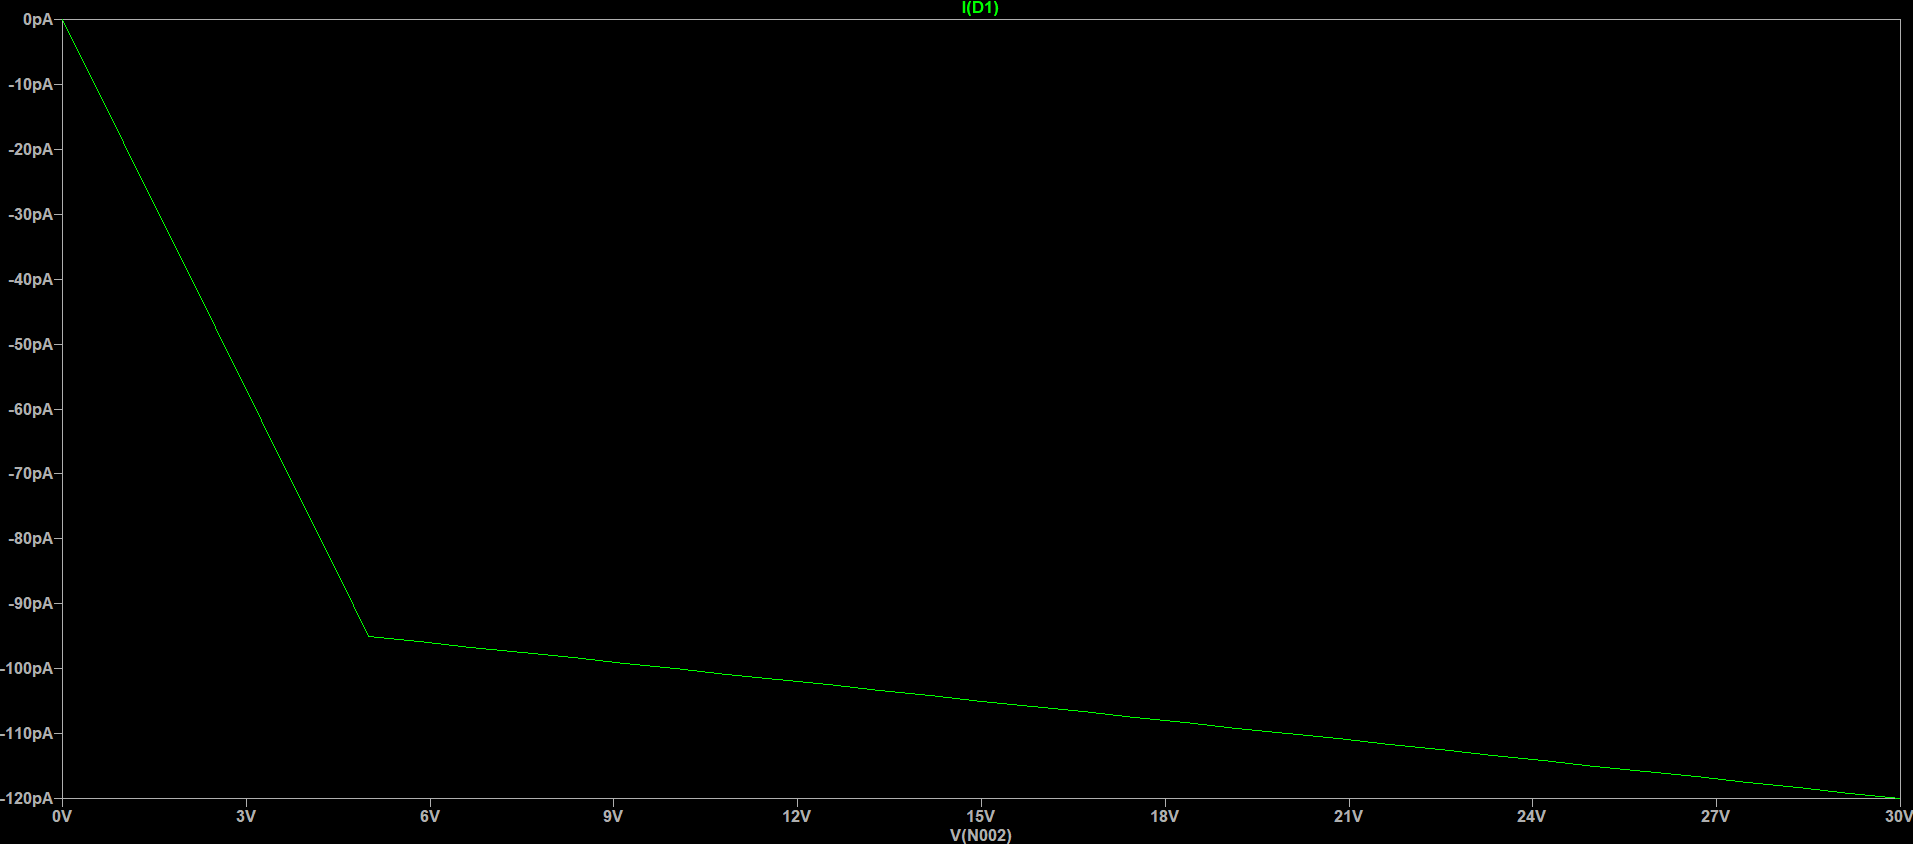
\includegraphics[width=0.75\textwidth]{../DIODE_REVERSE/0-30v.png}
    \caption{PN Diode Reverse Characteristic ($0\text{ V}$ to $30\text{ V}$).}
    \label{fig:diode_rev_sim}
\end{figure}

\subsection{Experimental Observations (PN Diode)}
\begin{table}[H]
\centering
\caption{PN Junction Diode (1N4007) Forward and Reverse Bias Tabulated Readings}
\begin{tabular}{c c c c | c c c}
\toprule
\multicolumn{4}{c|}{\textbf{Forward Bias}} & \multicolumn{3}{c}{\textbf{Reverse Bias}} \\
\midrule
\textbf{S.No.} & \textbf{$V_{sup}$ (V)} & \textbf{$V_f$ (V)} & \textbf{$I_f$ (mA)} & \textbf{S.No.} & \textbf{$V_{sup} = V_r$ (V)} & \textbf{$I_r$ ($\mu$A)} \\
\midrule
1  & 0.00 & 0.00 & 0.000 & 1 & 0.0 & 0.0 \\
2  & 0.40 & 0.40 & 0.006 & 2 & -5.0 & 0.0 \\
3  & 0.55 & 0.48 & 0.070 & 3 & -10.0 & 0.0 \\
4  & 0.65 & 0.51 & 0.140 & 4 & -15.0 & 0.0 \\
5  & 0.75 & 0.53 & 0.220 & 5 & -20.0 & 0.0 \\
6  & 2.88 & 0.63 & 2.220 & 6 & -25.0 & 0.0 \\
7  & 4.93 & 0.66 & 4.220 & 7 & -30.0 & 0.0 \\
8  & 6.97 & 0.68 & 6.220 & & & \\
9  & 11.04 & 0.70 & 10.220 & & & \\
10 & 15.11 & 0.72 & 14.220 & & & \\
11 & 20.97 & 0.73 & 20.000 & & & \\
\bottomrule
\end{tabular}
\end{table}

\subsection{Experimental V--I Characteristics \& Plots}
The experimental readings were plotted using Matplotlib in both linear scale ($I$ vs $V$) and semi-log scale ($\log|I|$ vs $V$).

\begin{figure}[H]
    \centering
    \begin{subfigure}[b]{0.48\textwidth}
        \centering
        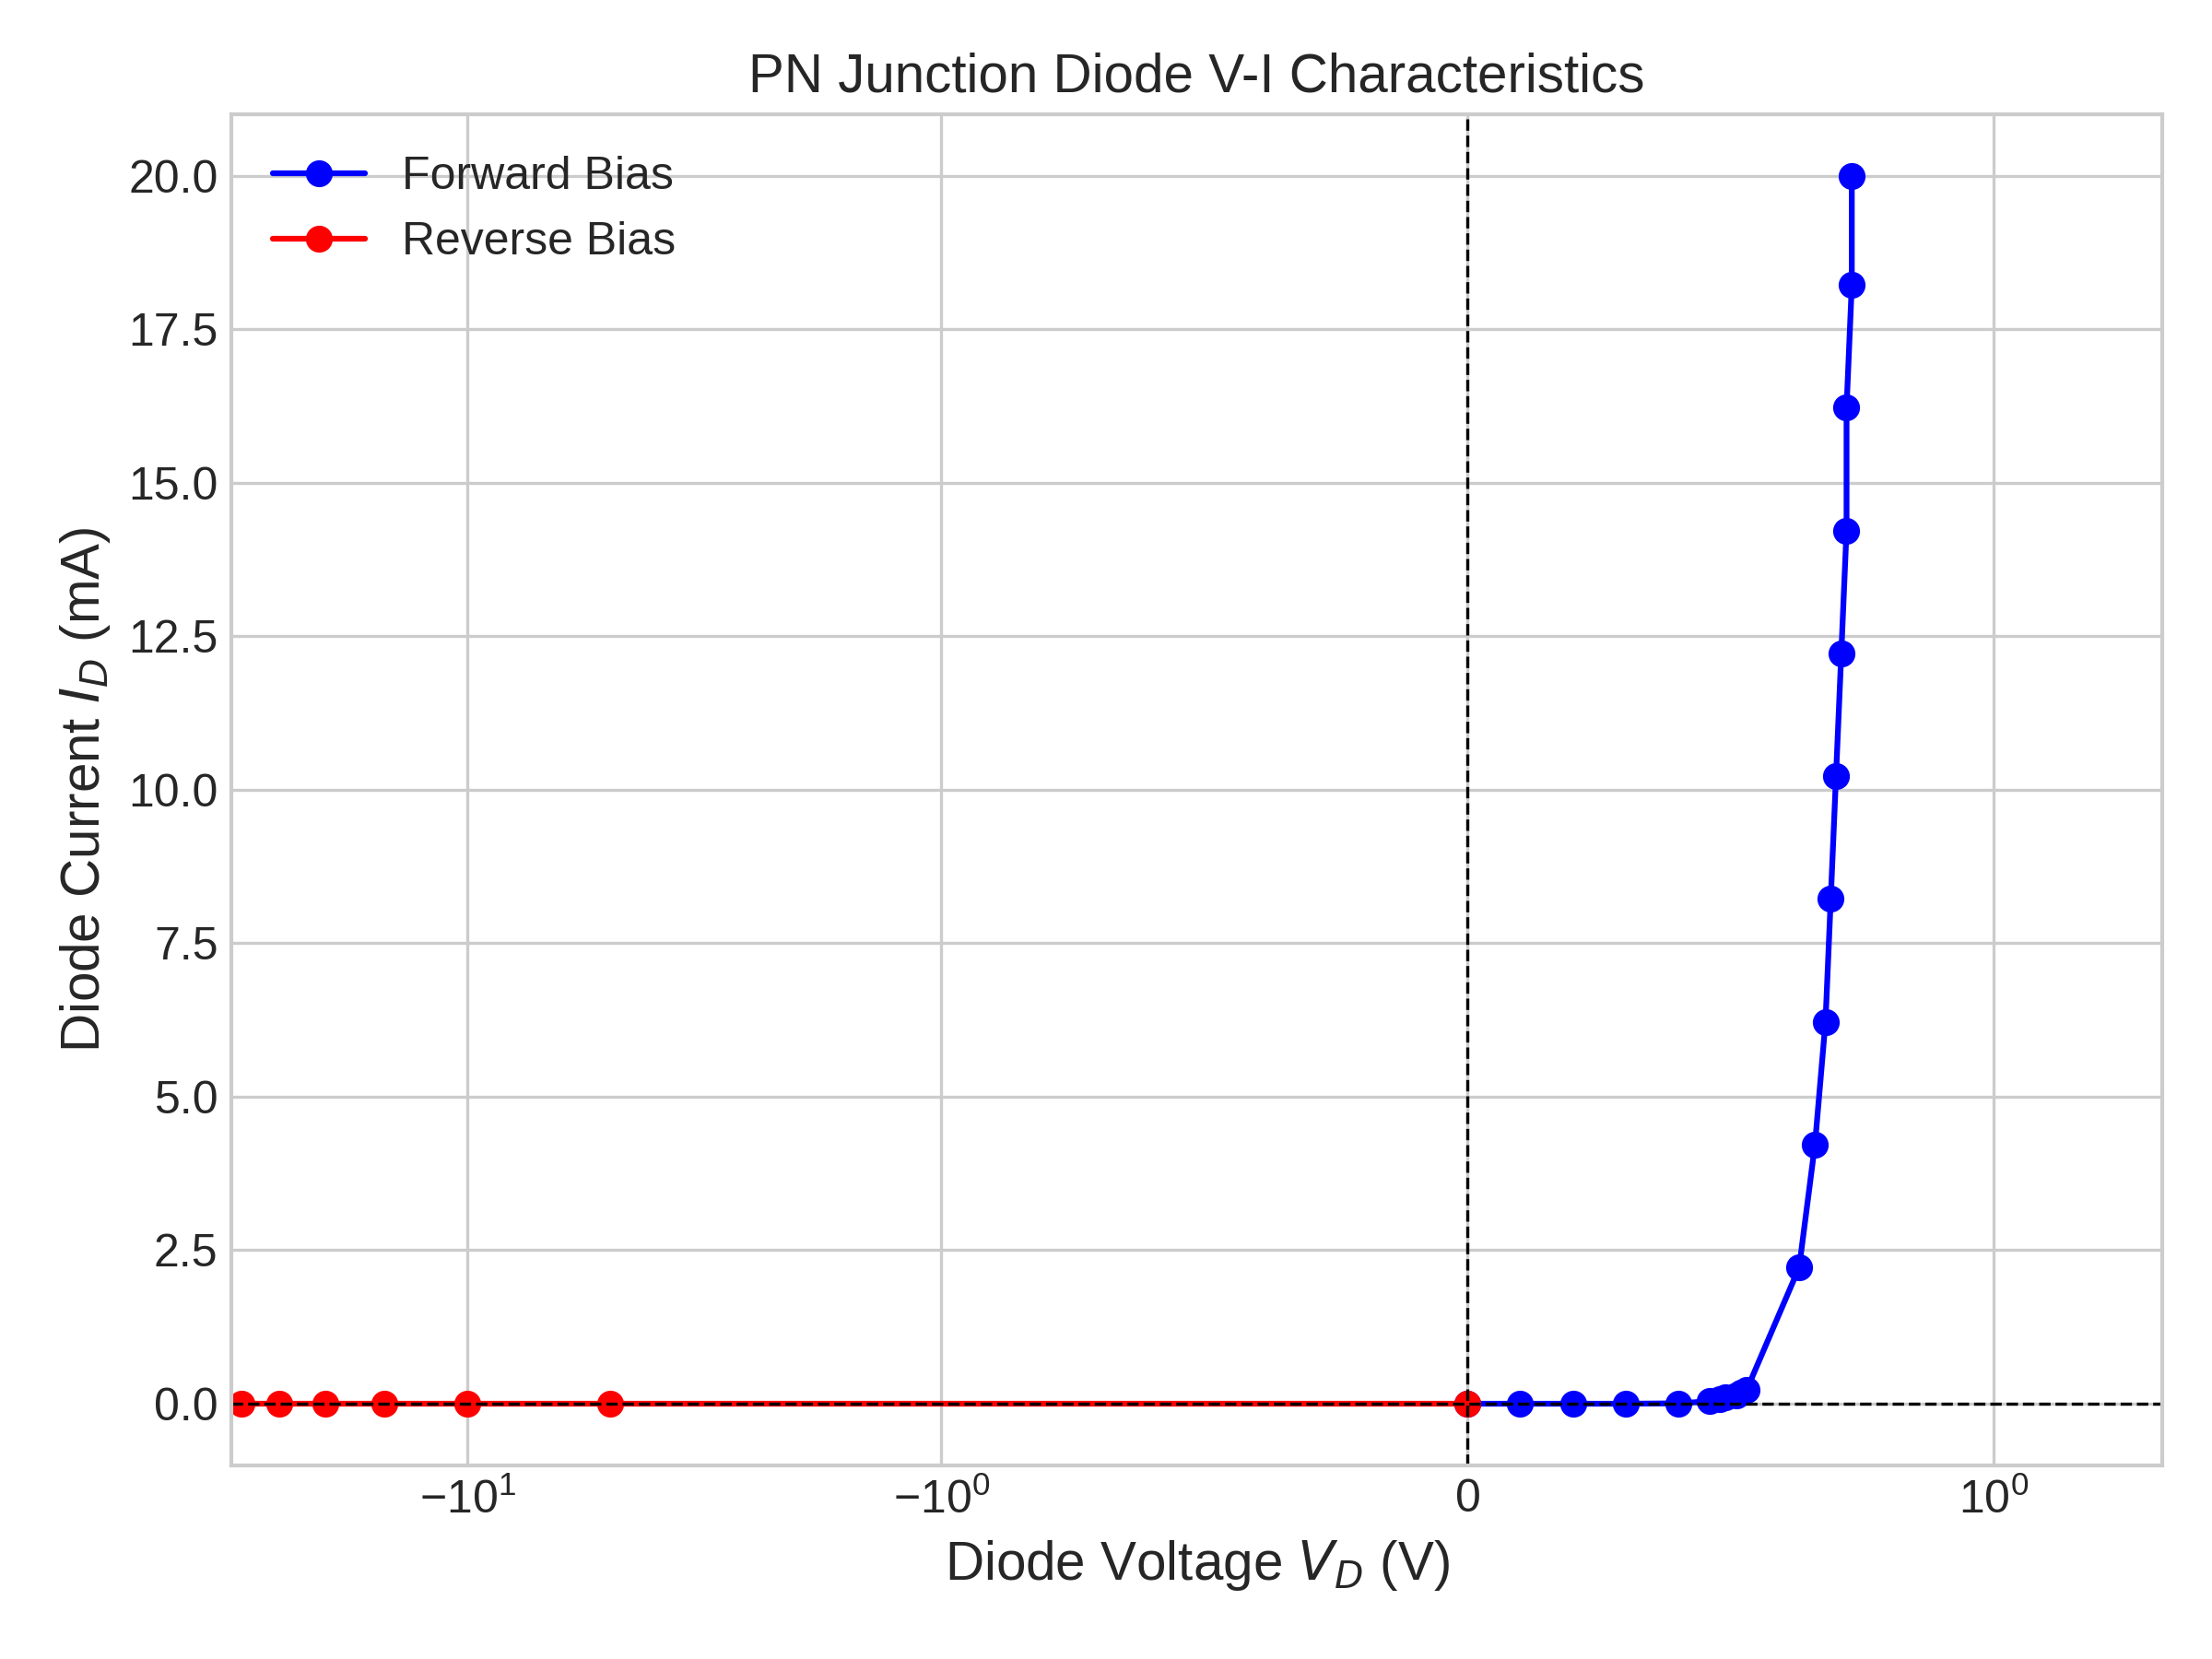
\includegraphics[width=\textwidth]{../DIODE_READINGS/pn_diode_vi_linear.png}
        \caption{Linear Scale Plot ($I$ vs $V$)}
    \end{subfigure}
    \hfill
    \begin{subfigure}[b]{0.48\textwidth}
        \centering
        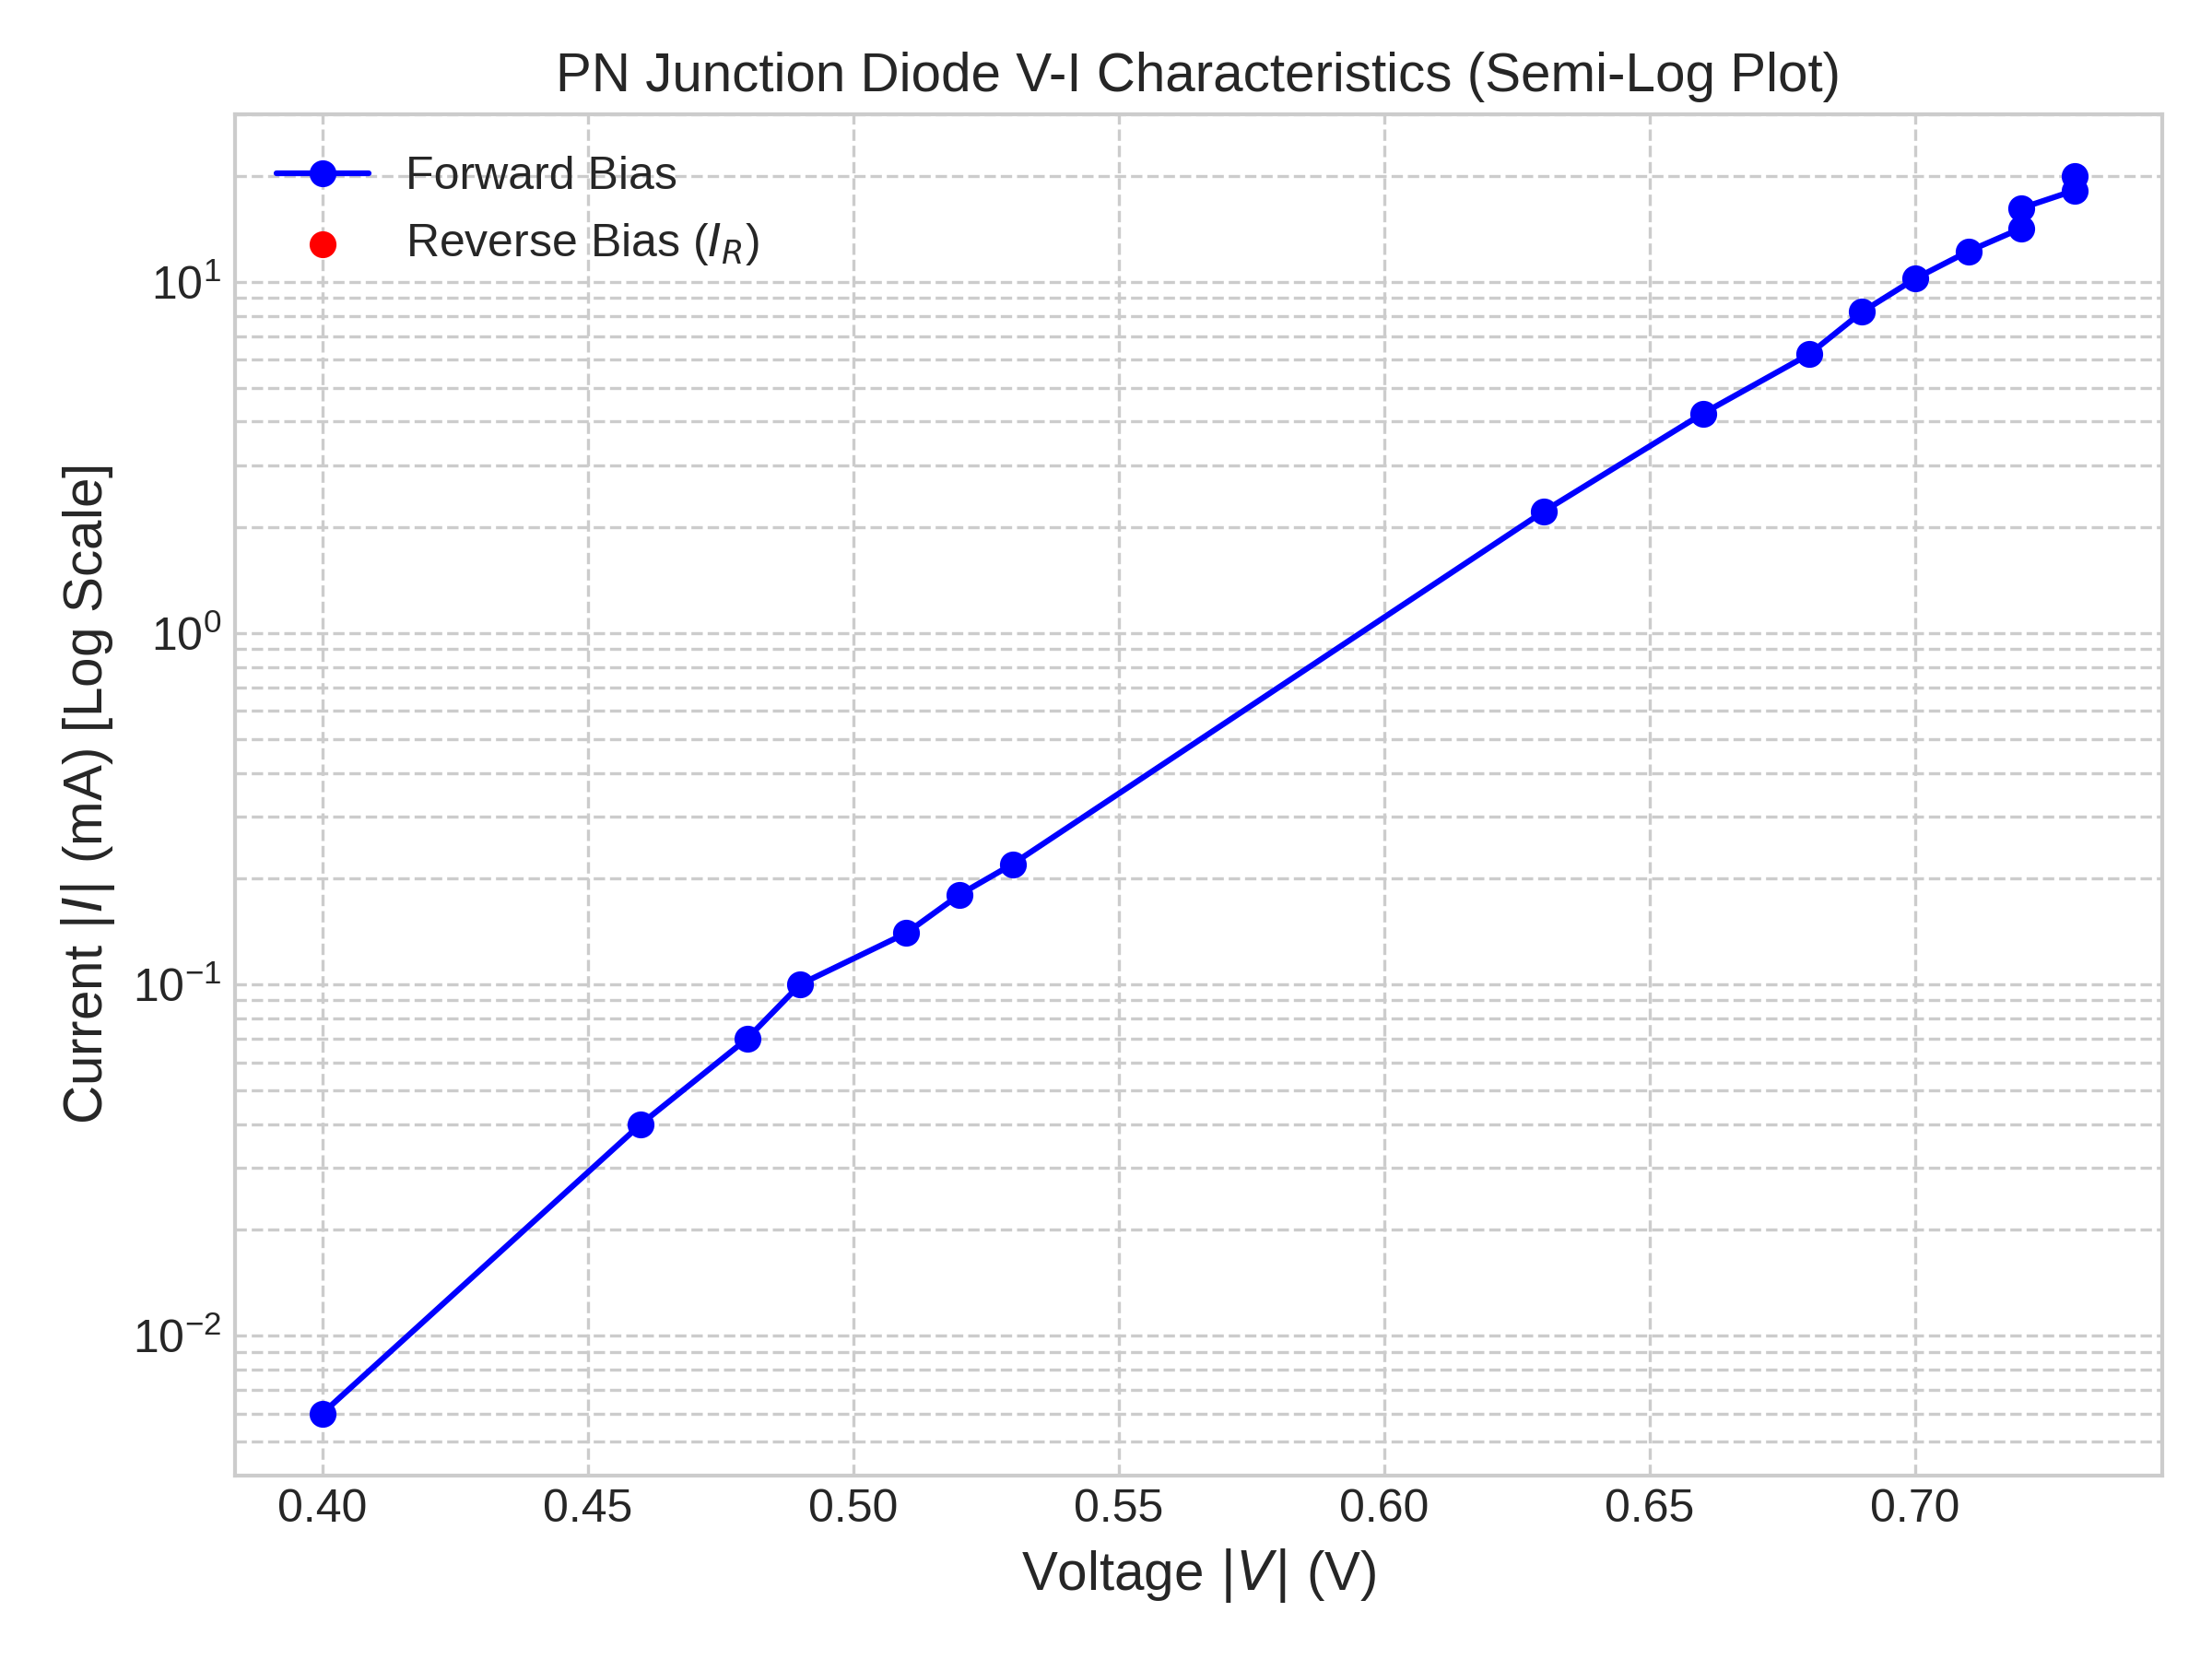
\includegraphics[width=\textwidth]{../DIODE_READINGS/pn_diode_vi_semilog.png}
        \caption{Semi-Log Plot ($\log|I|$ vs $V$)}
    \end{subfigure}
    \caption{Experimental $V$--$I$ Characteristic Curves for PN Junction Diode (1N4007).}
    \label{fig:pn_diode_exp_plots}
\end{figure}

\begin{figure}[H]
    \centering
    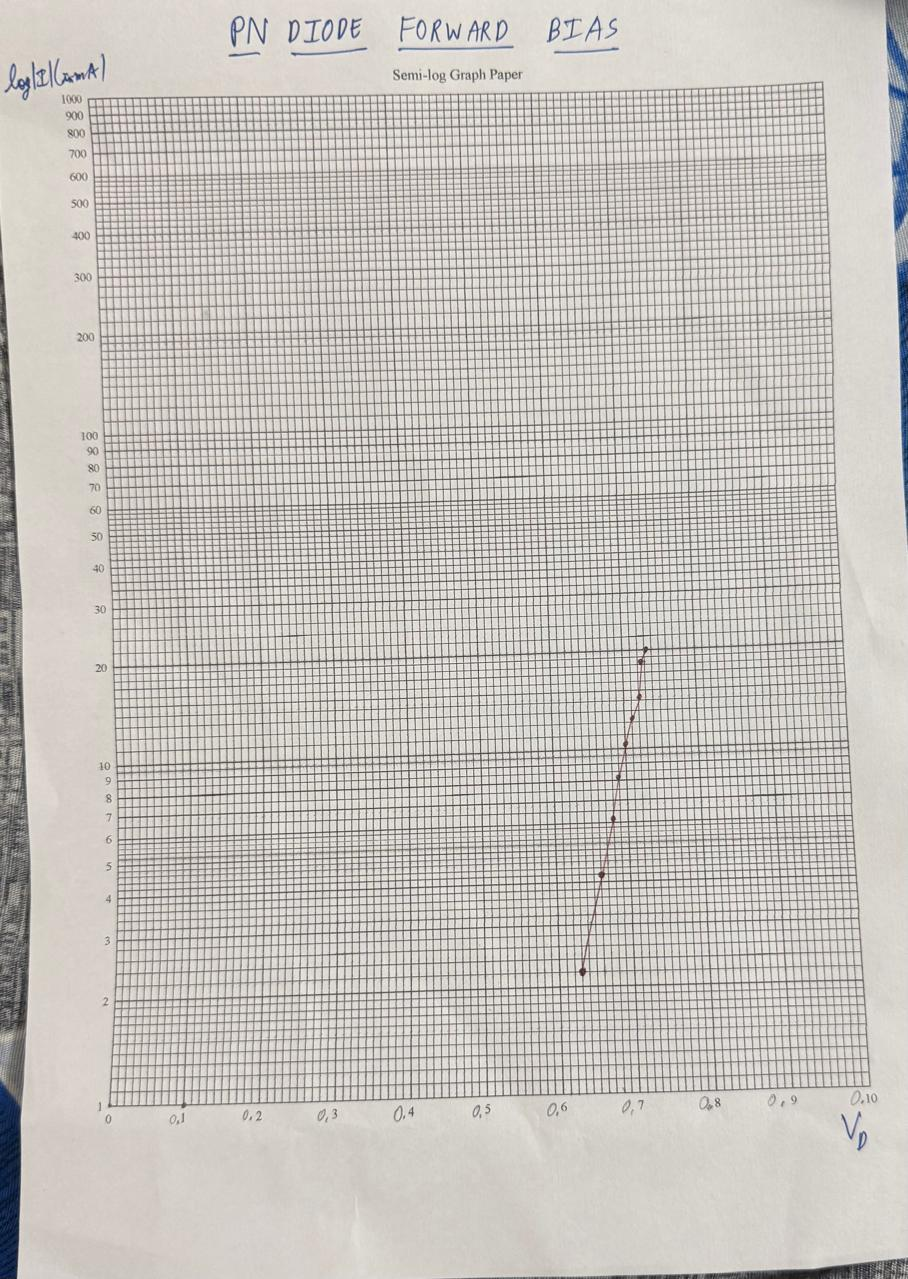
\includegraphics[width=0.5\textwidth]{../GRAPHS/diode_forward.jpeg}
    \caption{Graph-Paper Plot of the Forward-Bias $V$--$I$ Characteristics of PN Junction Diode.}
    \label{fig:pn_diode_graph_plot}
\end{figure}

\newpage

\subsection{Calculated Parameters (PN Diode)}
\begin{itemize}
    \item \textbf{Cut-in Voltage (\boldmath{$V_\gamma$}):} \textbf{$\approx 0.60\text{ V}$} (exponential current rise begins above $0.6\text{ V}$).
    \item \textbf{Static Forward Resistance (\boldmath{$R_{DC} = V_f / I_f$}):}
    \begin{itemize}
        \item At $I_f = 2.22\text{ mA}, V_f = 0.63\text{ V}$: \textbf{$R_{DC} = \frac{0.63}{2.22\text{ mA}} = 283.78\text{ }\Omega$}.
        \item At $I_f = 4.22\text{ mA}, V_f = 0.66\text{ V}$: \textbf{$R_{DC} = \frac{0.66}{4.22\text{ mA}} = 156.40\text{ }\Omega$}.
        \item At $I_f = 10.22\text{ mA}, V_f = 0.70\text{ V}$: \textbf{$R_{DC} = \frac{0.70}{10.22\text{ mA}} = 68.49\text{ }\Omega$}.
        \item At $I_f = 20.0\text{ mA}, V_f = 0.73\text{ V}$: \textbf{$R_{DC} = \frac{0.73}{20.0\text{ mA}} = 36.50\text{ }\Omega$}.
    \end{itemize}
    \item \textbf{Dynamic Forward Resistance (\boldmath{$r_d = \Delta V_f / \Delta I_f$}):}
    \begin{itemize}
        \item In knee region ($2.22\text{ mA}$ to $4.22\text{ mA}$): \textbf{$r_d = \frac{0.66 - 0.63}{4.22\text{ mA} - 2.22\text{ mA}} = \frac{0.03\text{ V}}{2\text{ mA}} = 15.00\text{ }\Omega$}.
        \item In high-conduction region ($10.22\text{ mA}$ to $20.0\text{ mA}$): \textbf{$r_d = \frac{0.73 - 0.70}{20.0\text{ mA} - 10.22\text{ mA}} = \frac{0.03\text{ V}}{9.78\text{ mA}} = 3.07\text{ }\Omega$}.
    \end{itemize}
    \item \textbf{Reverse Saturation Current (\boldmath{$I_s$}):} \textbf{$I_s < 1\text{ }\mu\text{A}$} ($0\text{ mA}$ measured from $0\text{ V}$ to $30\text{ V}$).
\end{itemize}


\section{Part B: Zener Diode Characteristics}

\subsection{Theoretical Background}
A Zener diode is designed to operate safely in reverse breakdown (\textbf{$V_Z$}). Once in breakdown, the terminal voltage remains virtually constant over a wide range of reverse currents. In forward bias, it behaves as a normal PN junction diode.

\subsection{Circuit Diagrams and Simulation Waveforms}

\subsubsection{Zener Diode -- Forward Bias}
\begin{figure}[H]
    \centering
    
\includegraphics[width=0.65\textwidth]{../ZENER_FORWARD/circuit.png}
    \caption{Zener Diode Forward Bias Circuit Schematic.}
    \label{fig:zener_fwd_circuit}
\end{figure}

\begin{figure}[H]
    \centering
    \begin{subfigure}[b]{0.48\textwidth}
        \centering
        
\includegraphics[width=\textwidth]{../ZENER_FORWARD/0-0.5v.png}
        \caption{Sub-knee Region ($0\text{ V}$ to $0.5\text{ V}$)}
    \end{subfigure}
    \hfill
    \begin{subfigure}[b]{0.48\textwidth}
        \centering
        
\includegraphics[width=\textwidth]{../ZENER_FORWARD/0.5-0.75v.png}
        \caption{Conduction Region ($0.5\text{ V}$ to $0.75\text{ V}$)}
    \end{subfigure}
    \caption{Zener Diode Forward Bias Simulation Plots.}
    \label{fig:zener_fwd_sim}
\end{figure}

\subsubsection{Zener Diode -- Reverse Bias and Breakdown}
\begin{figure}[H]
    \centering
    
\includegraphics[width=0.65\textwidth]{../ZENER_REVERSE/circuit.png}
    \caption{Zener Diode Reverse Bias Circuit Schematic.}
    \label{fig:zener_rev_circuit}
\end{figure}

\begin{figure}[H]
    \centering
    \begin{subfigure}[b]{0.32\textwidth}
        \centering
        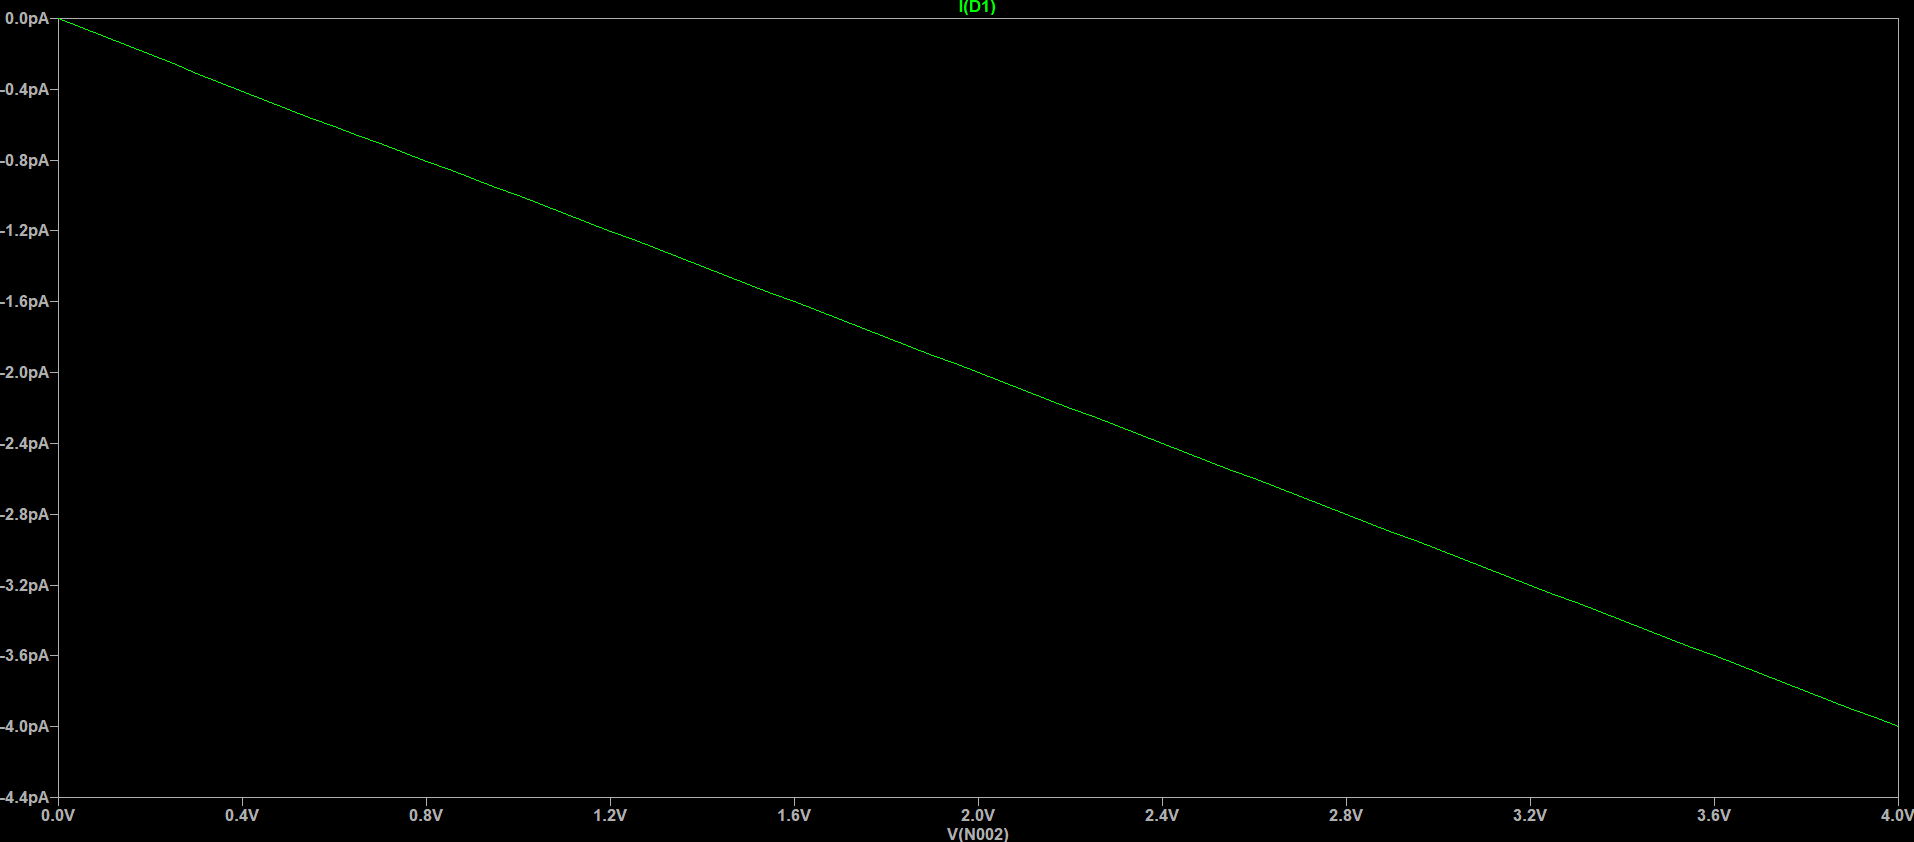
\includegraphics[width=\textwidth]{../ZENER_REVERSE/0-4v.png}
        \caption{Pre-breakdown ($0\text{--}4\text{ V}$)}
    \end{subfigure}
    \hfill
    \begin{subfigure}[b]{0.32\textwidth}
        \centering
        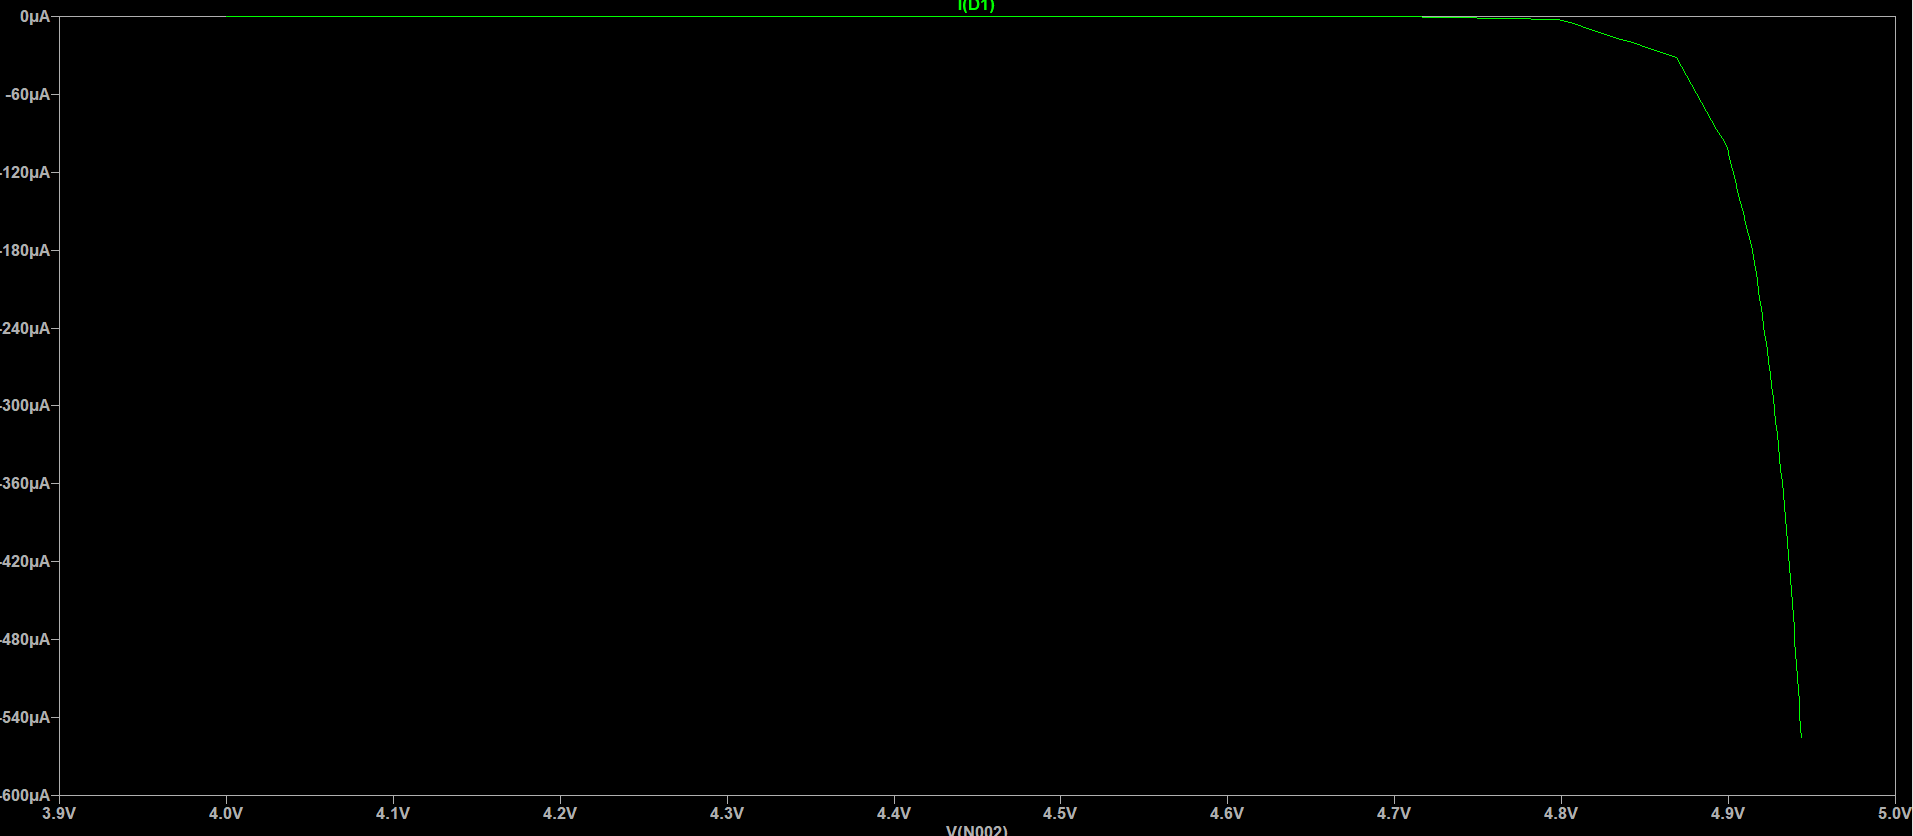
\includegraphics[width=\textwidth]{../ZENER_REVERSE/4-5.5v.png}
        \caption{Breakdown Knee ($4\text{--}5.5\text{ V}$)}
    \end{subfigure}
    \hfill
    \begin{subfigure}[b]{0.32\textwidth}
        \centering
        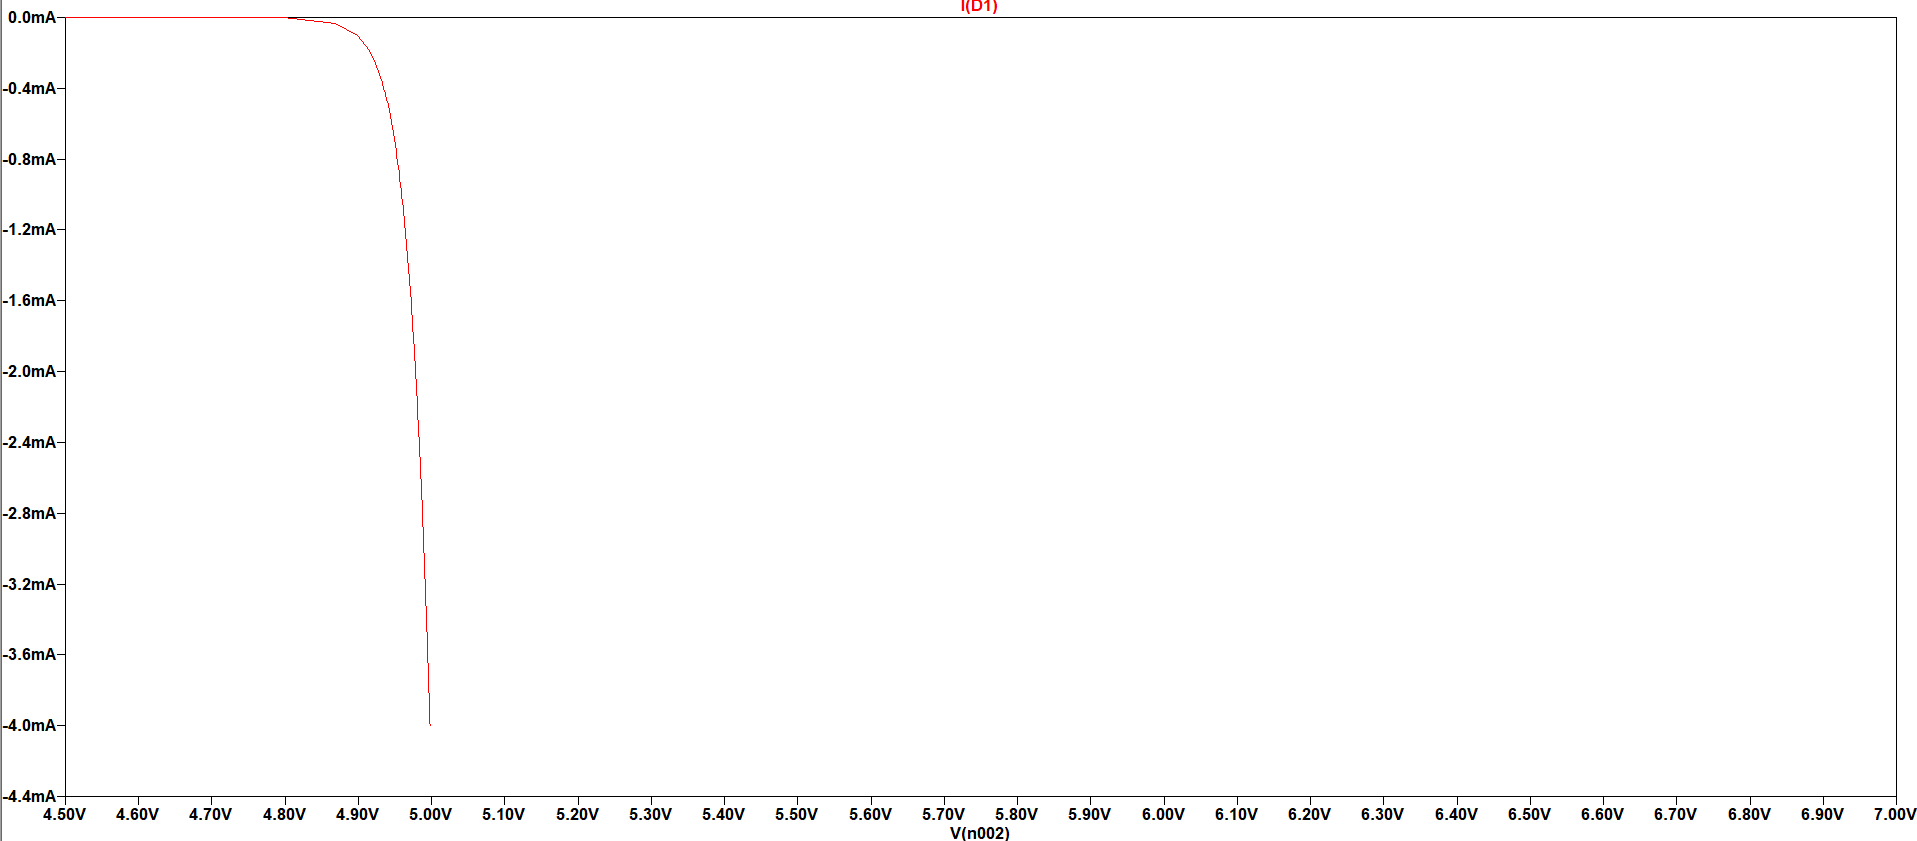
\includegraphics[width=\textwidth]{../ZENER_REVERSE/5.5+v.png}
        \caption{Zener Region ($> 5.5\text{ V}$)}
    \end{subfigure}
    \caption{Zener Diode Reverse Breakdown Simulation Response.}
    \label{fig:zener_rev_sim}
\end{figure}

\subsection{Experimental Observations (Zener Diode)}
\begin{table}[H]
\centering
\caption{Zener Diode (1N4733A) Forward and Reverse Bias Tabulated Readings}
\begin{tabular}{c c c c | c c c c}
\toprule
\multicolumn{4}{c|}{\textbf{Forward Bias}} & \multicolumn{4}{c}{\textbf{Reverse Breakdown Bias}} \\
\midrule
\textbf{S.No.} & \textbf{$V_{sup}$ (V)} & \textbf{$V_f$ (V)} & \textbf{$I_f$ (mA)} & \textbf{S.No.} & \textbf{$V_{sup}$ (V)} & \textbf{$V_r$ (V)} & \textbf{$I_r$ (mA)} \\
\midrule
1 & 0.00 & 0.00 & 0.000 & 1  & 0.00   & 0.00  & 0.000 \\
2 & 0.10 & 0.10 & 0.000 & 2  & -1.00  & -1.00 & 0.000 \\
3 & 0.30 & 0.30 & 0.000 & 3  & -2.50  & -2.50 & -0.001 \\
4 & 0.50 & 0.50 & 0.000 & 4  & -3.50  & -3.48 & -0.020 \\
5 & 0.55 & 0.55 & 0.002 & 5  & -4.10  & -4.00 & -0.100 \\
6 & 0.60 & 0.59 & 0.008 & 6  & -4.70  & -4.40 & -0.300 \\
7 & 0.65 & 0.62 & 0.025 & 7  & -5.10  & -4.58 & -0.520 \\
8 & 0.70 & 0.65 & 0.050 & 8  & -5.50  & -4.70 & -0.800 \\
9 & 0.75 & 0.66 & 0.090 & 9  & -14.04 & -5.17 & -8.800 \\
  &      &      &       & 10 & -25.43 & -5.25 & -20.000 \\
\bottomrule
\end{tabular}
\end{table}

\subsection{Experimental V--I Characteristics \& Plots}
\begin{figure}[H]
    \centering
    \begin{subfigure}[b]{0.48\textwidth}
        \centering
        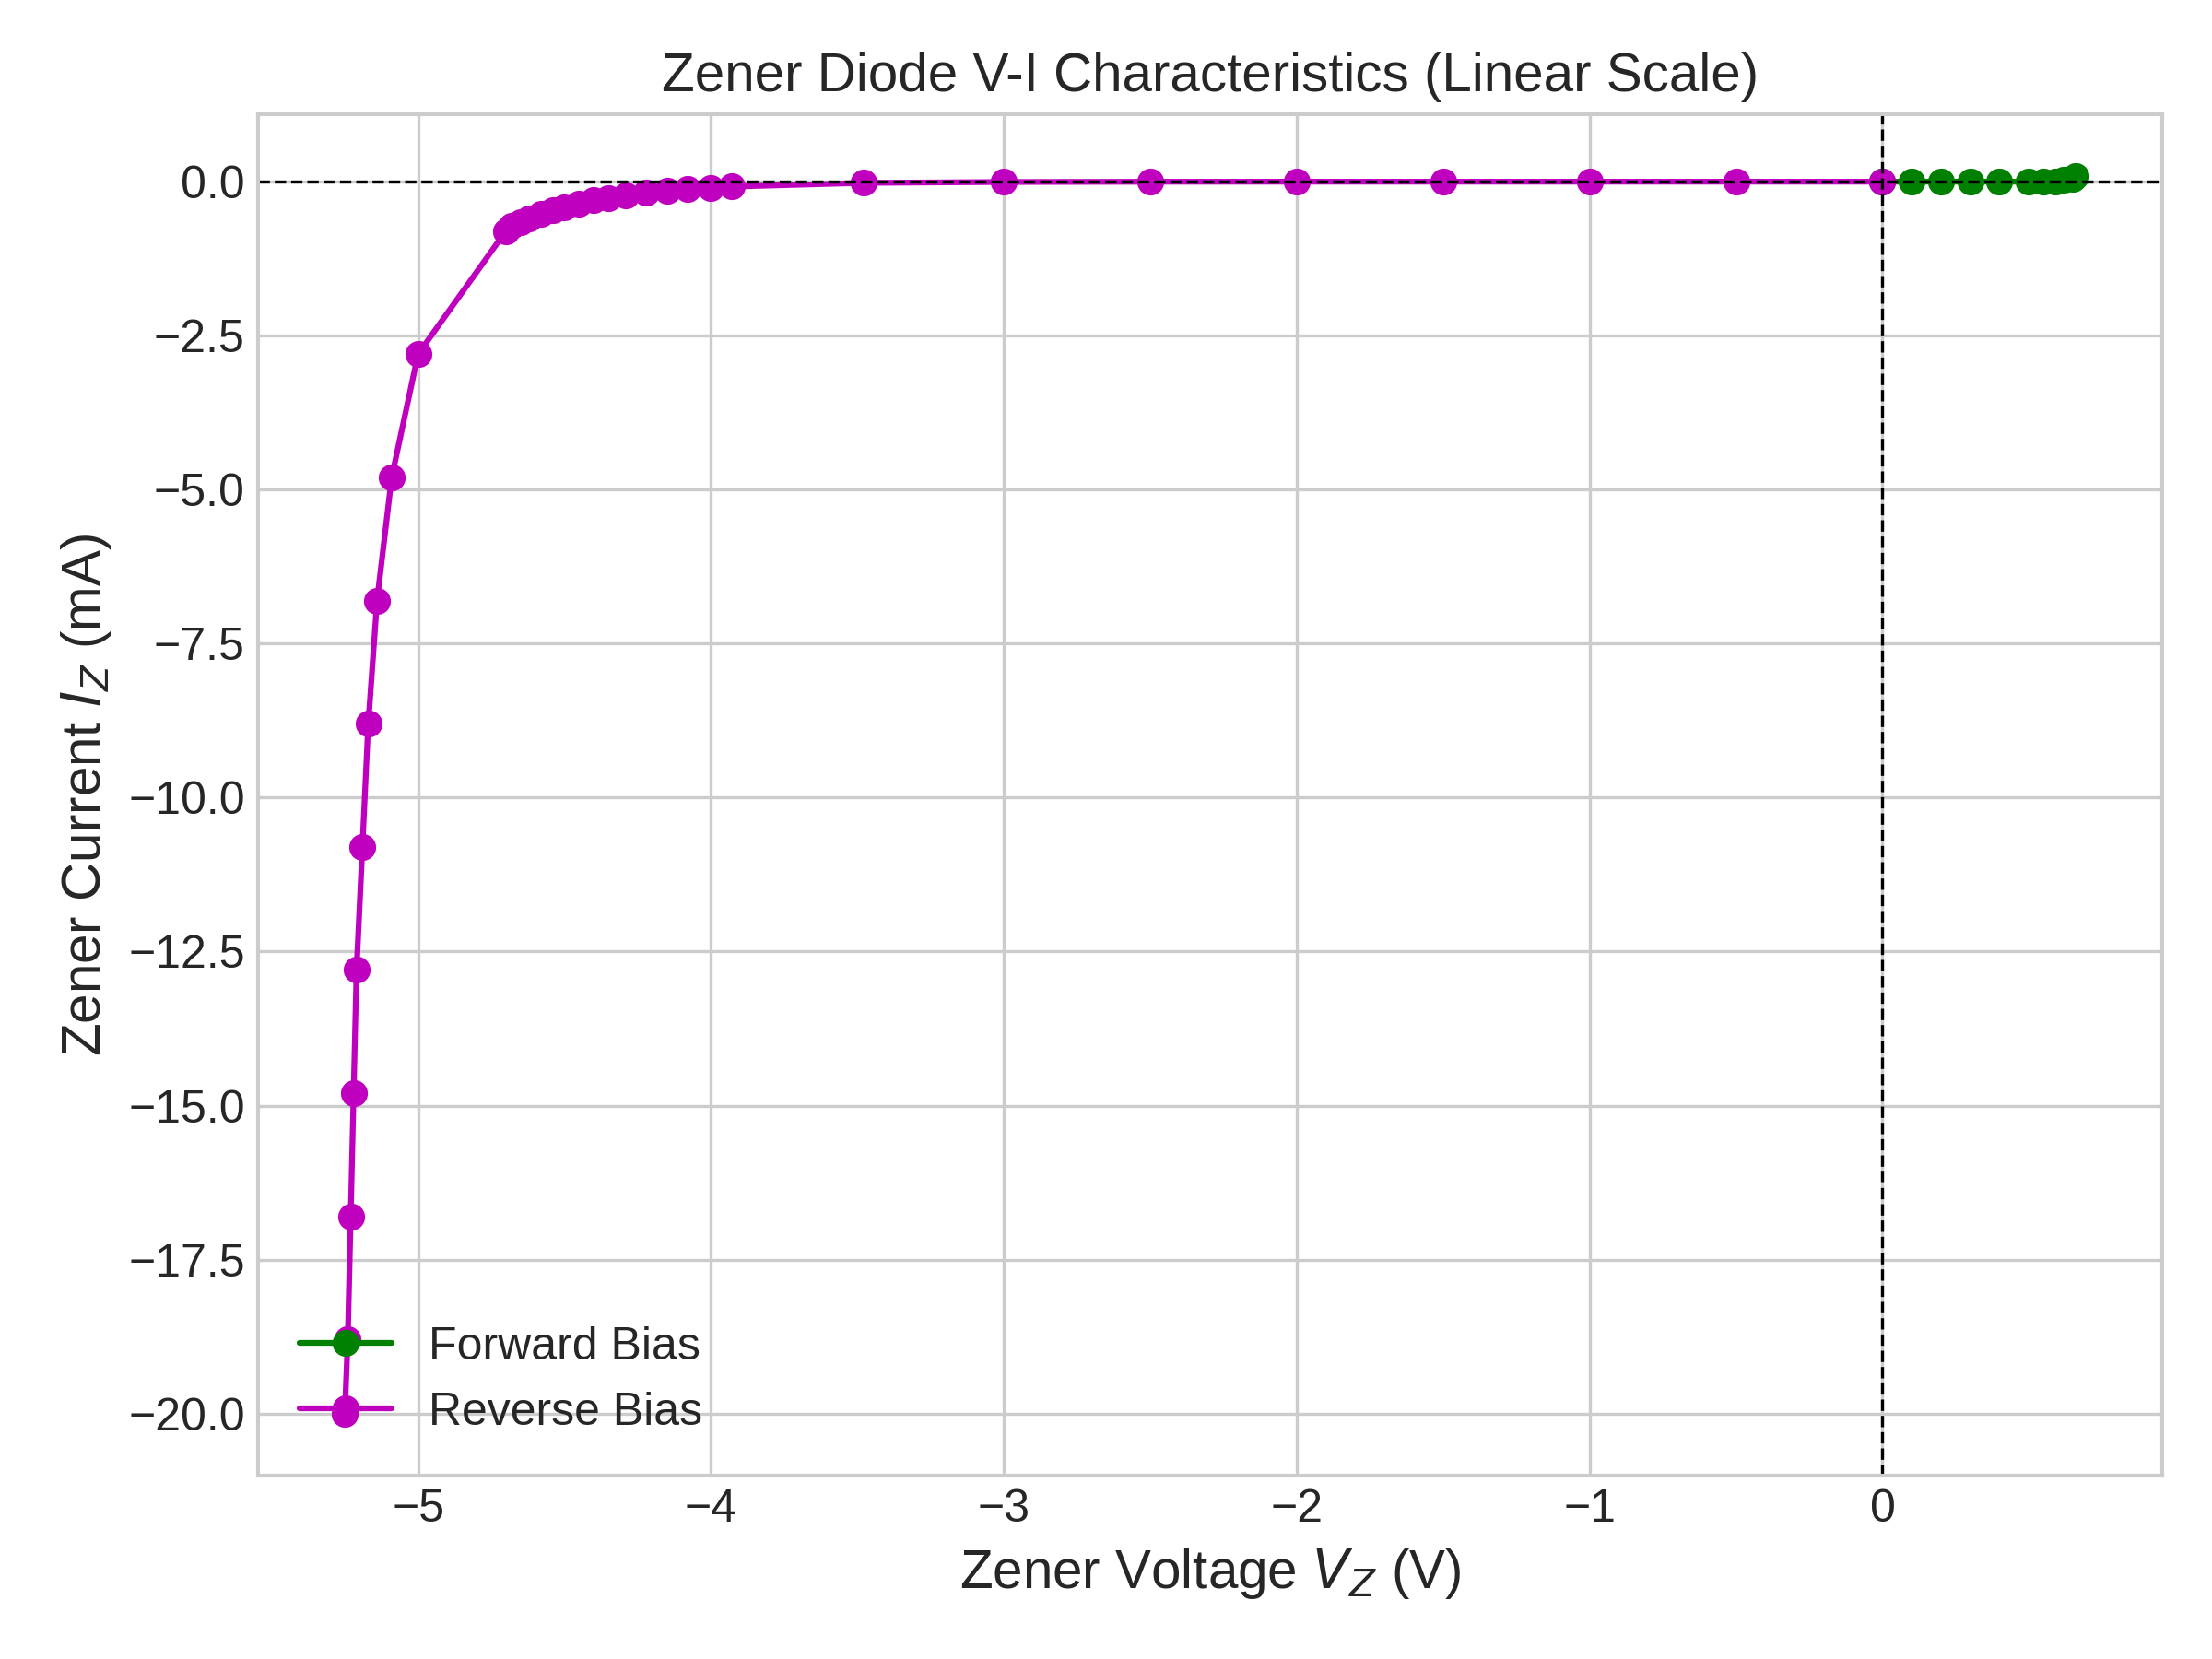
\includegraphics[width=\textwidth]{../ZENER_FORWARD_READINGS/zener_diode_vi_linear.png}
        \caption{Linear Scale Plot ($I$ vs $V$)}
    \end{subfigure}
    \hfill
    \begin{subfigure}[b]{0.48\textwidth}
        \centering
        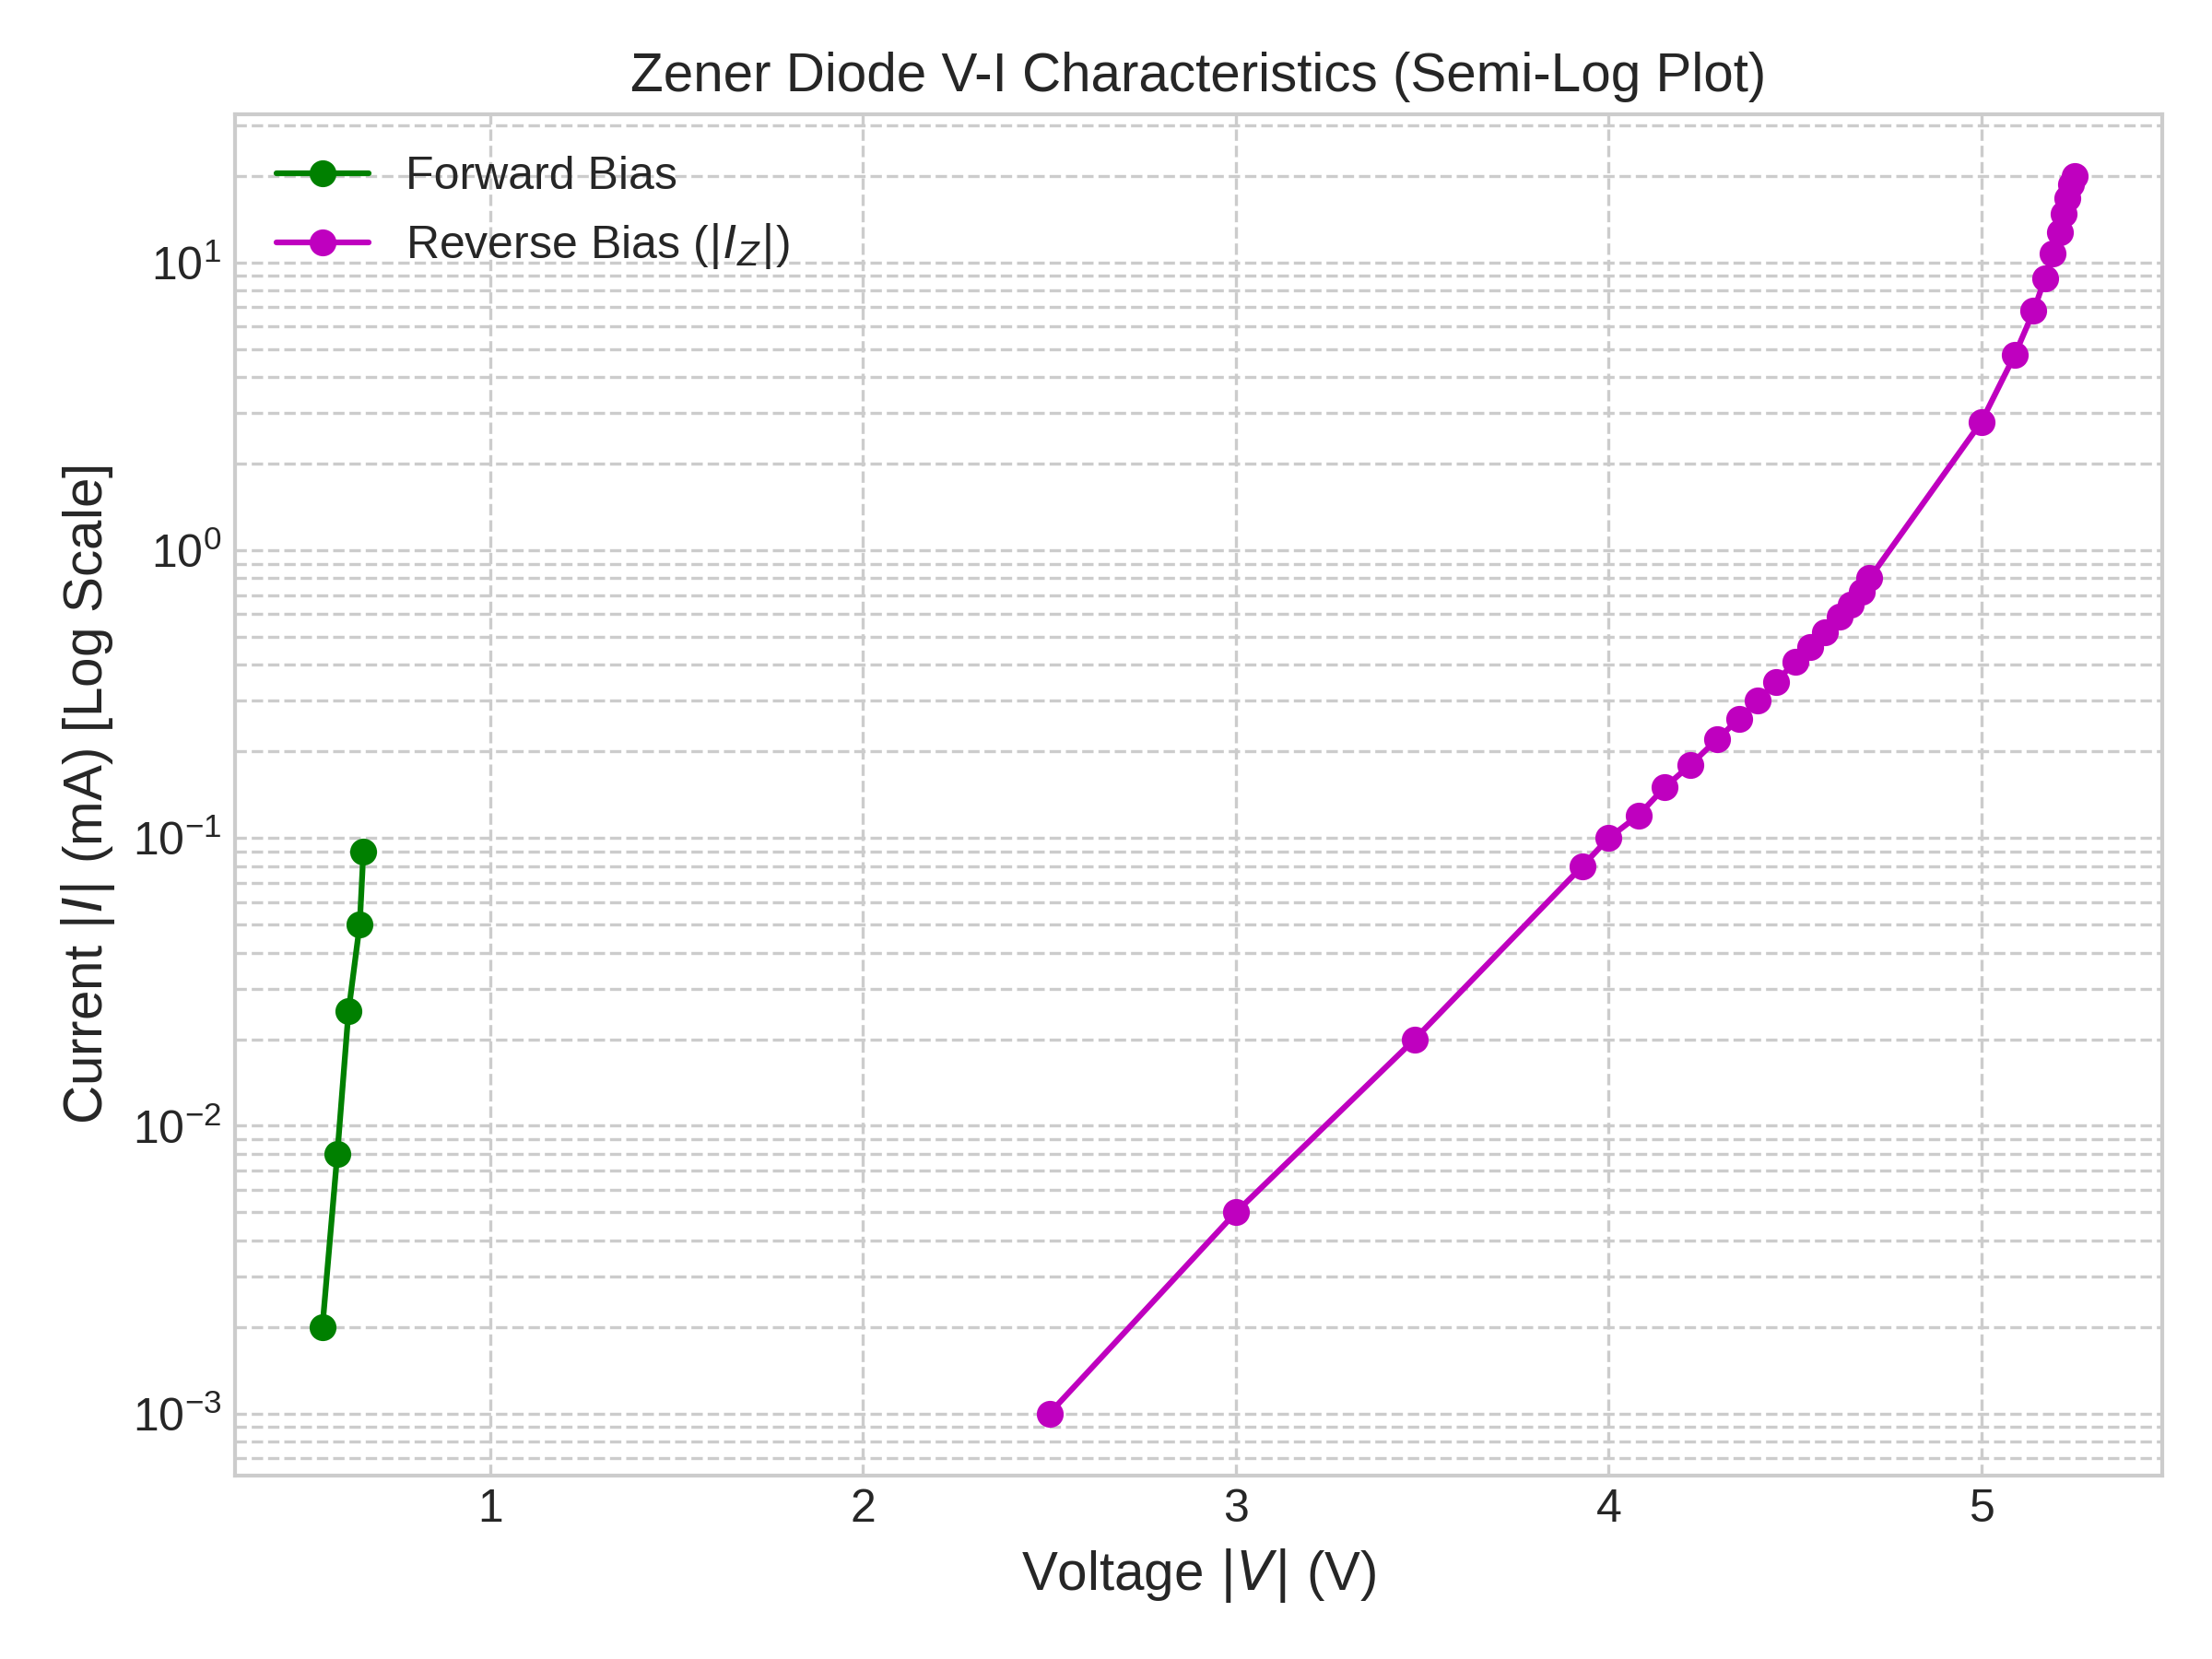
\includegraphics[width=\textwidth]{../ZENER_FORWARD_READINGS/zener_diode_vi_semilog.png}
        \caption{Semi-Log Plot ($\log|I|$ vs $V$)}
    \end{subfigure}
    \caption{Experimental $V$--$I$ Characteristic Curves for Zener Diode (1N4733A).}
    \label{fig:zener_diode_exp_plots}
\end{figure}

\begin{figure}[H]
    \centering
    \begin{subfigure}[b]{0.42\textwidth}
        \centering
        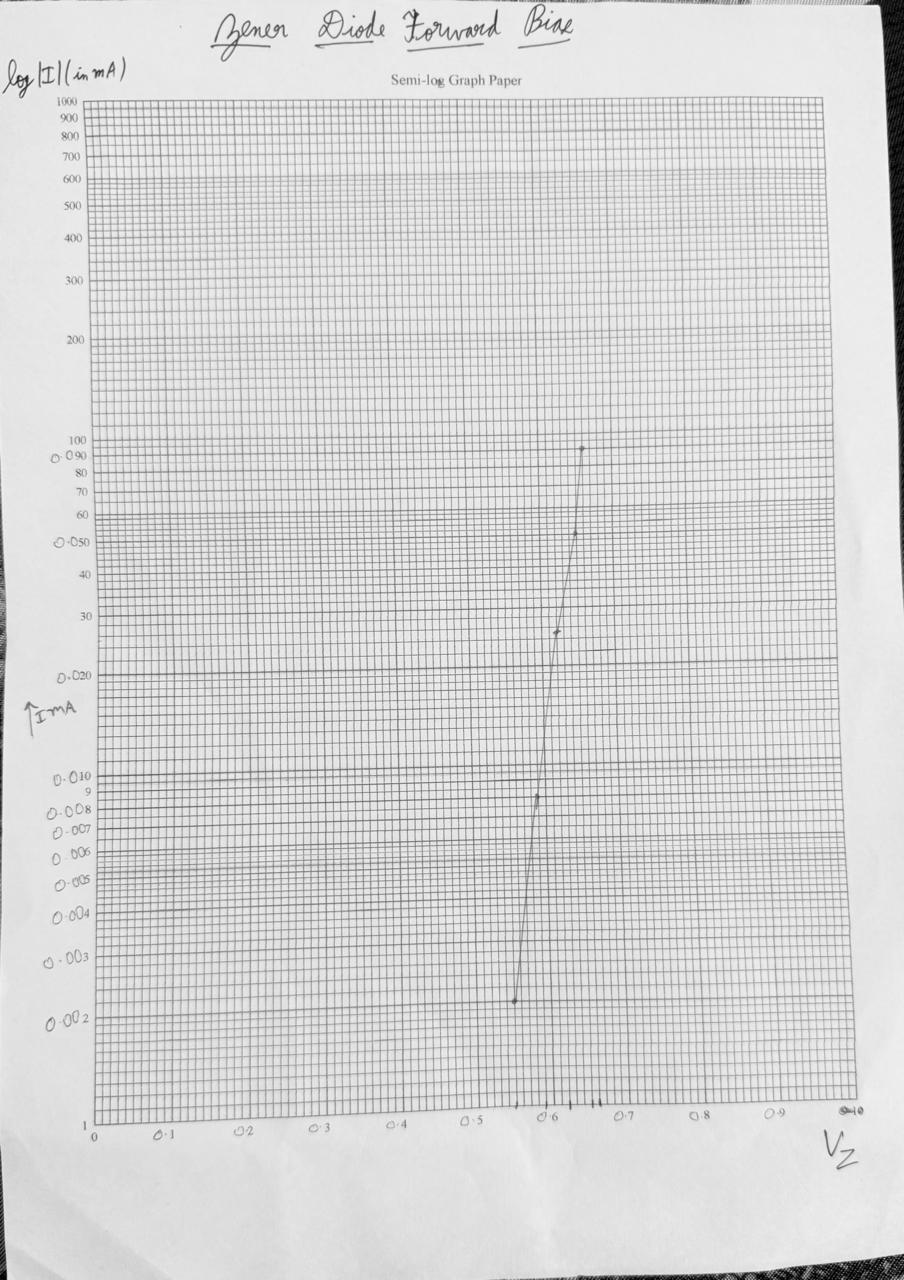
\includegraphics[width=\textwidth]{../GRAPHS/zener_forward.jpeg}
        \caption{Graph-Paper Plot of the Forward-Bias $V$--$I$ Characteristics.}
    \end{subfigure}
    \hfill
    \begin{subfigure}[b]{0.42\textwidth}
        \centering
        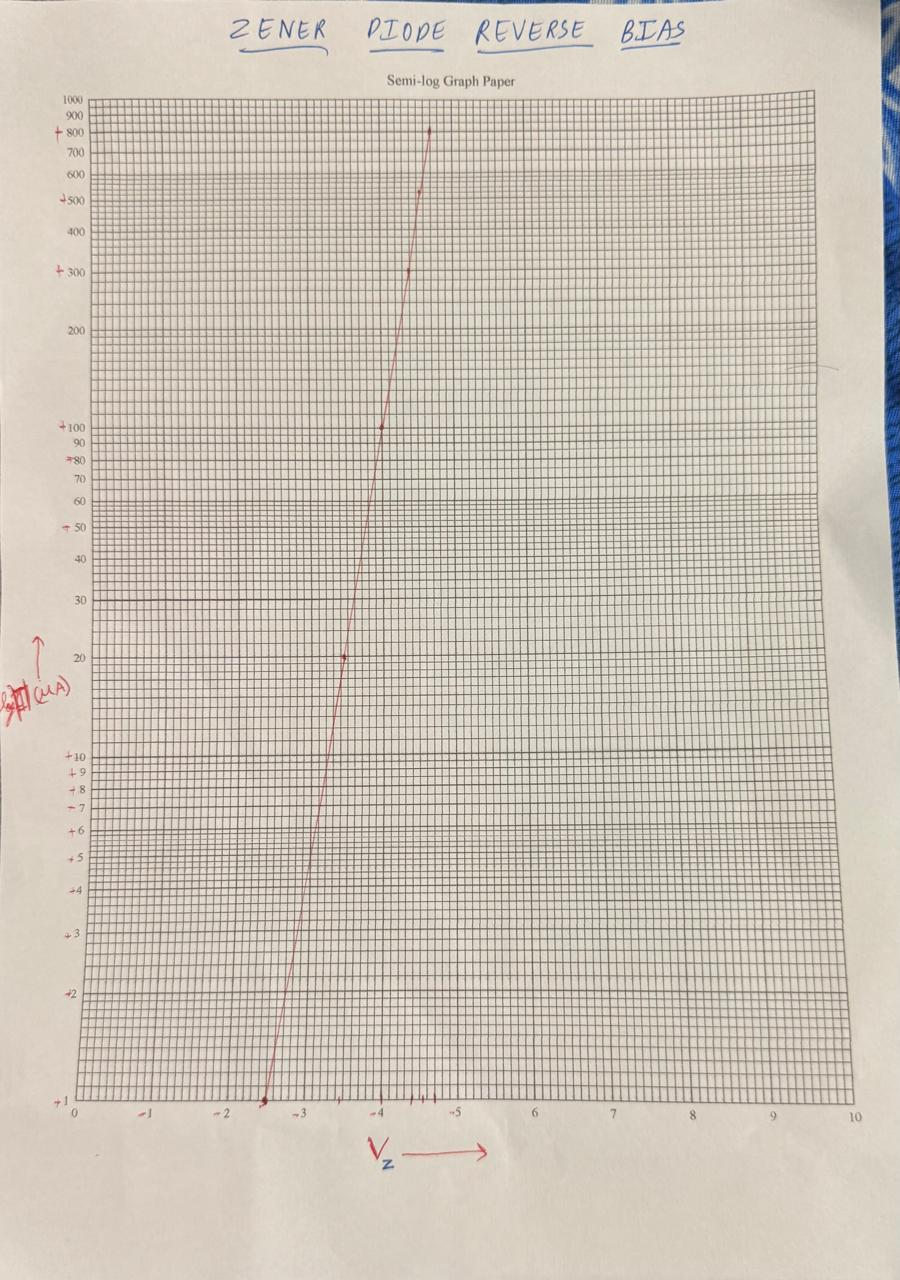
\includegraphics[width=\textwidth]{../GRAPHS/zener_reverse.jpeg}
        \caption{Graph-Paper Plot of the Reverse-Bias $V$--$I$ Characteristics.}
    \end{subfigure}
    \caption{Graph-Paper Plots for Zener Diode (1N4733A).}
    \label{fig:zener_diode_graph_plots}
\end{figure}

\subsection{Calculated Parameters (Zener Diode)}
\begin{itemize}
    \item \textbf{Zener Breakdown Voltage (\boldmath{$V_Z$}):} \textbf{Breakdown starts at $V_Z \approx 5.00\text{ V}$ and stabilizes up to $5.25\text{ V}$ at $20\text{ mA}$}.
    \item \textbf{Zener Dynamic Resistance (\boldmath{$R_Z = \Delta V_Z / \Delta I_Z$}):}
    \begin{equation}
    \mathbf{R_Z = \frac{5.25\text{ V} - 5.00\text{ V}}{20.0\text{ mA} - 2.8\text{ mA}} = \frac{0.25\text{ V}}{17.2\text{ mA}} = 14.53\text{ }\Omega}
    \end{equation}
\end{itemize}

\newpage
\section{Part C: Diode Clipper Circuits}

\subsection{Theoretical Background}
Clippers remove portions of an applied signal above or below chosen reference levels without distorting the remainder. A load resistor of $R_L = 100\text{ k}\Omega$ was connected across the output to ensure smooth DSO readings and eliminate loading effects.

\subsection{Circuit Diagrams, Simulations \& Hardware DSO Waveforms}

\subsubsection{Positive Clipper (Clipping above +1 V reference)}
In positive clipping, the diode conducts when $V_{in} > +1\text{ V} + V_\gamma$, holding output to $+1.60\text{ V}$.
\begin{figure}[H]
    \centering
    \begin{subfigure}[b]{0.32\textwidth}
        \centering
        
\includegraphics[width=\textwidth]{../POSITIVE_CLIPPER/circuit.png}
        \caption{Circuit Schematic}
    \end{subfigure}
    \hfill
    \begin{subfigure}[b]{0.32\textwidth}
        \centering
        
\includegraphics[width=\textwidth]{../POSITIVE_CLIPPER/sim.png}
        \caption{LTspice Simulation}
    \end{subfigure}
    \hfill
    \begin{subfigure}[b]{0.32\textwidth}
        \centering
        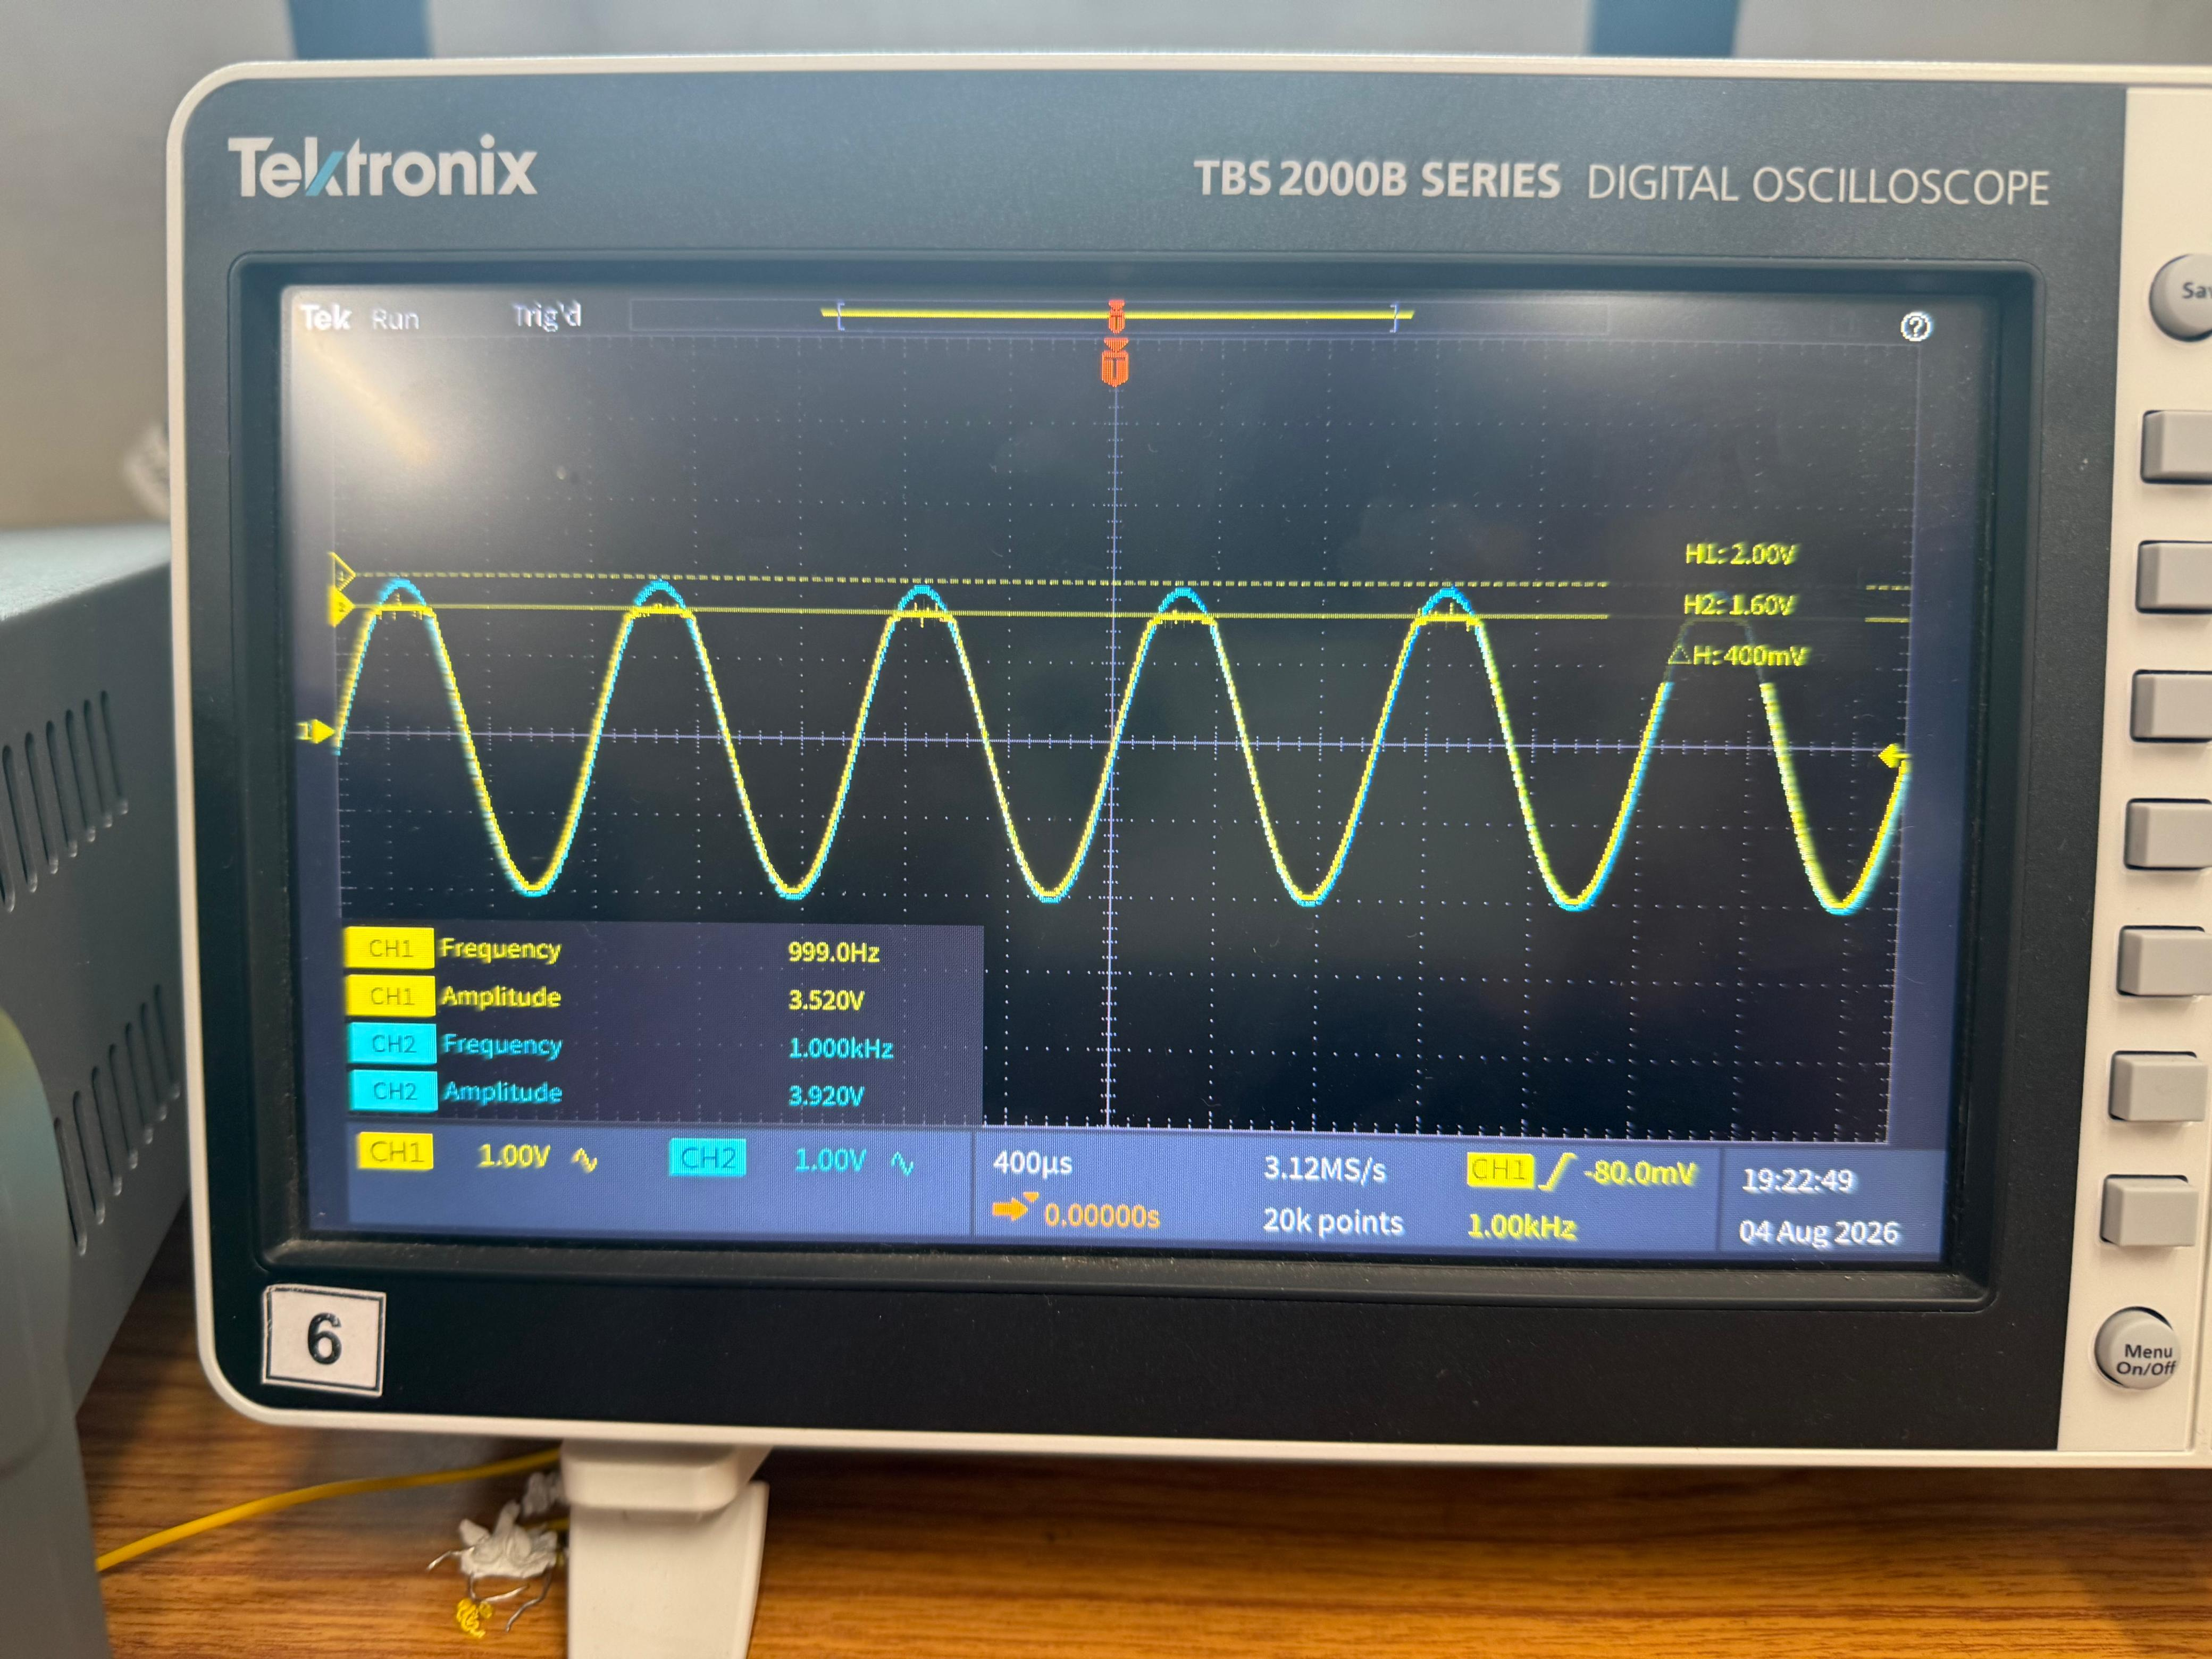
\includegraphics[width=\textwidth]{../POSITIVE_CLIPPER/dso_pos_clip.jpeg}
        \caption{DSO Trace}
    \end{subfigure}
    \caption{Positive Clipper Circuit, Simulation, and Measured DSO Waveform (Clipped at $+1.60\text{ V}$).}
    \label{fig:pos_clipper}
\end{figure}

\subsubsection{Negative Clipper (Clipping below -1 V reference)}
In negative clipping, the diode conducts when $V_{in} < -1\text{ V} - V_\gamma$, holding output to $-1.68\text{ V}$.
\begin{figure}[H]
    \centering
    \begin{subfigure}[b]{0.32\textwidth}
        \centering
        
\includegraphics[width=\textwidth]{../NEGATIVE_CLIPPER/circuit.png}
        \caption{Circuit Schematic}
    \end{subfigure}
    \hfill
    \begin{subfigure}[b]{0.32\textwidth}
        \centering
        
\includegraphics[width=\textwidth]{../NEGATIVE_CLIPPER/sim.png}
        \caption{LTspice Simulation}
    \end{subfigure}
    \hfill
    \begin{subfigure}[b]{0.32\textwidth}
        \centering
        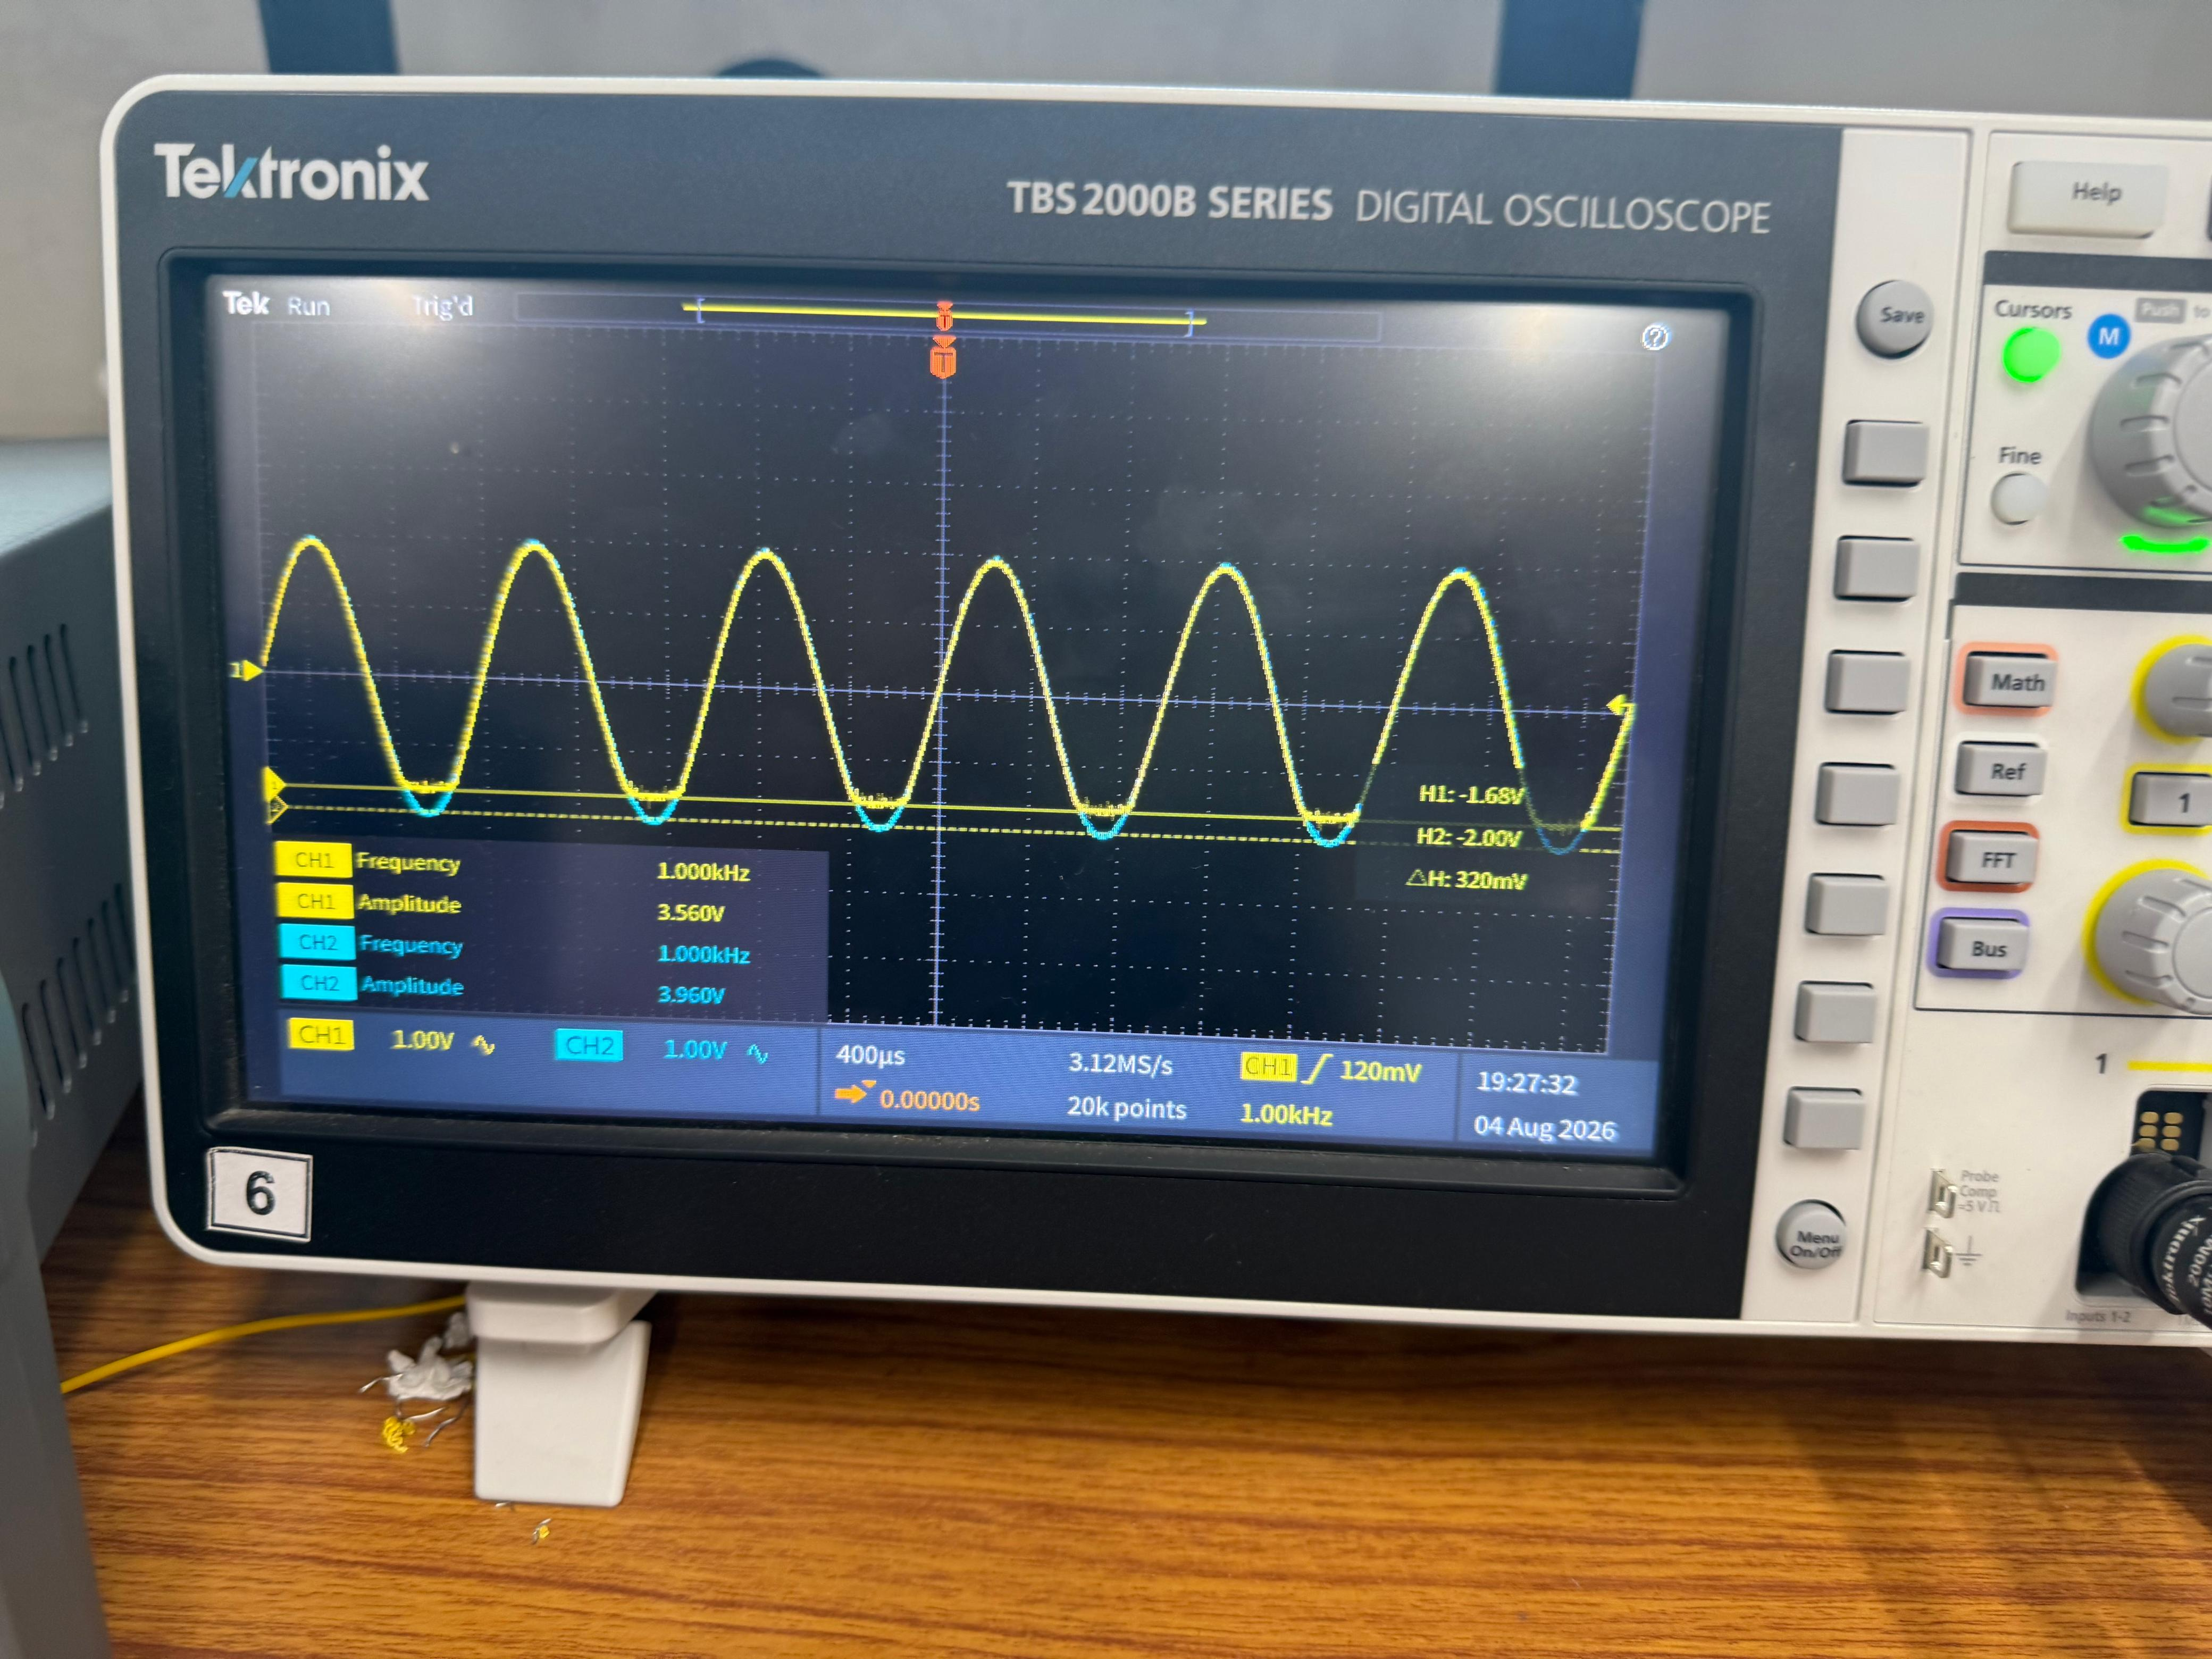
\includegraphics[width=\textwidth]{../NEGATIVE_CLIPPER/dso_neg_clip.jpeg}
        \caption{DSO Trace}
    \end{subfigure}
    \caption{Negative Clipper Circuit, Simulation, and Measured DSO Waveform (Clipped at $-1.68\text{ V}$).}
    \label{fig:neg_clipper}
\end{figure}

\newpage

\subsubsection{Biased Clipper (Two-Level Clipper)}
Both positive and negative peaks are clipped independently. The upper limit clipped at $+1.20\text{ V}$ and lower limit clipped at $-0.92\text{ V}$.
\begin{figure}[H]
    \centering
    \begin{subfigure}[b]{0.32\textwidth}
        \centering
        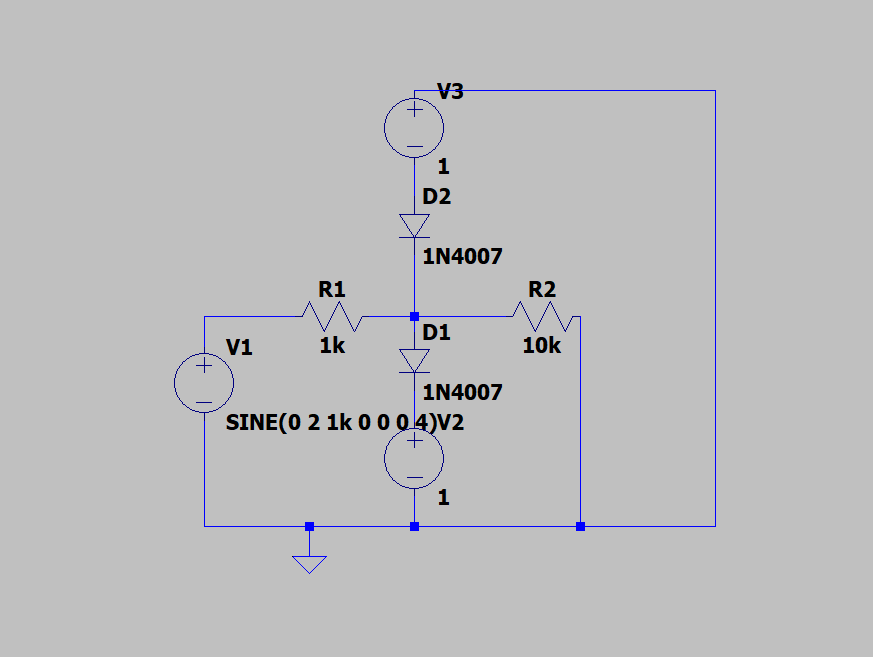
\includegraphics[width=\textwidth]{../BIASED_CLIPPER/circuit.png}
        \caption{Circuit Schematic}
    \end{subfigure}
    \hfill
    \begin{subfigure}[b]{0.32\textwidth}
        \centering
        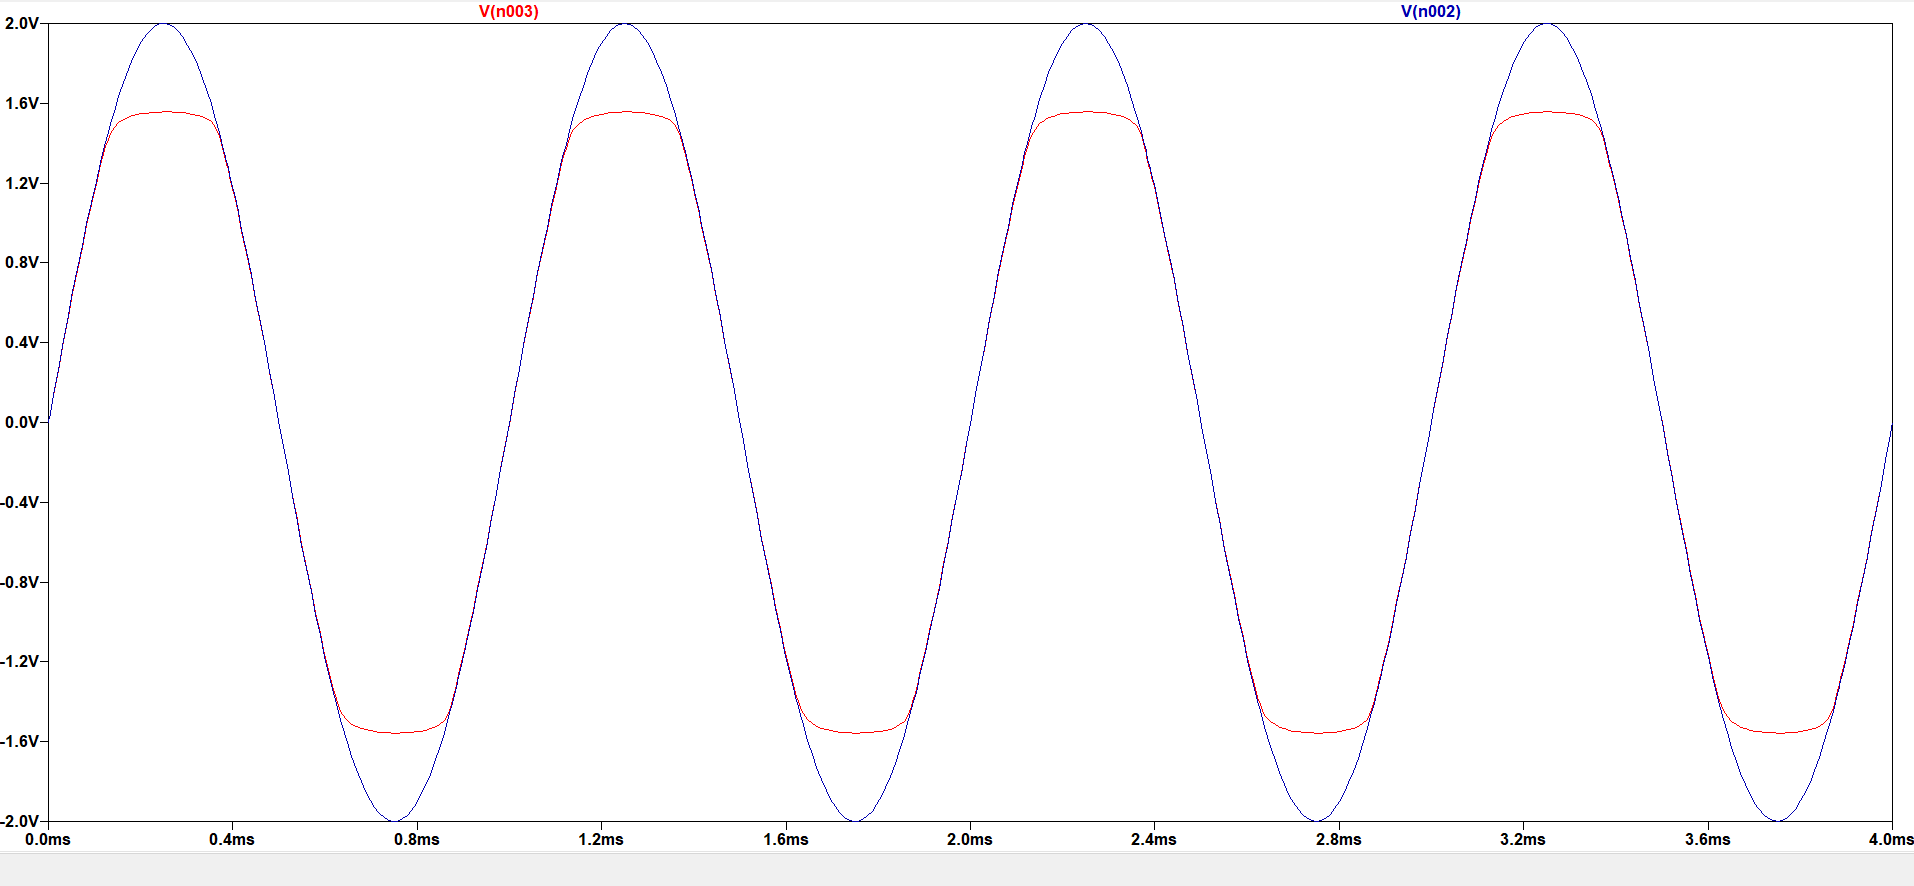
\includegraphics[width=\textwidth]{../BIASED_CLIPPER/sim.png}
        \caption{LTspice Simulation}
    \end{subfigure}
    \hfill
    \begin{subfigure}[b]{0.32\textwidth}
        \centering
        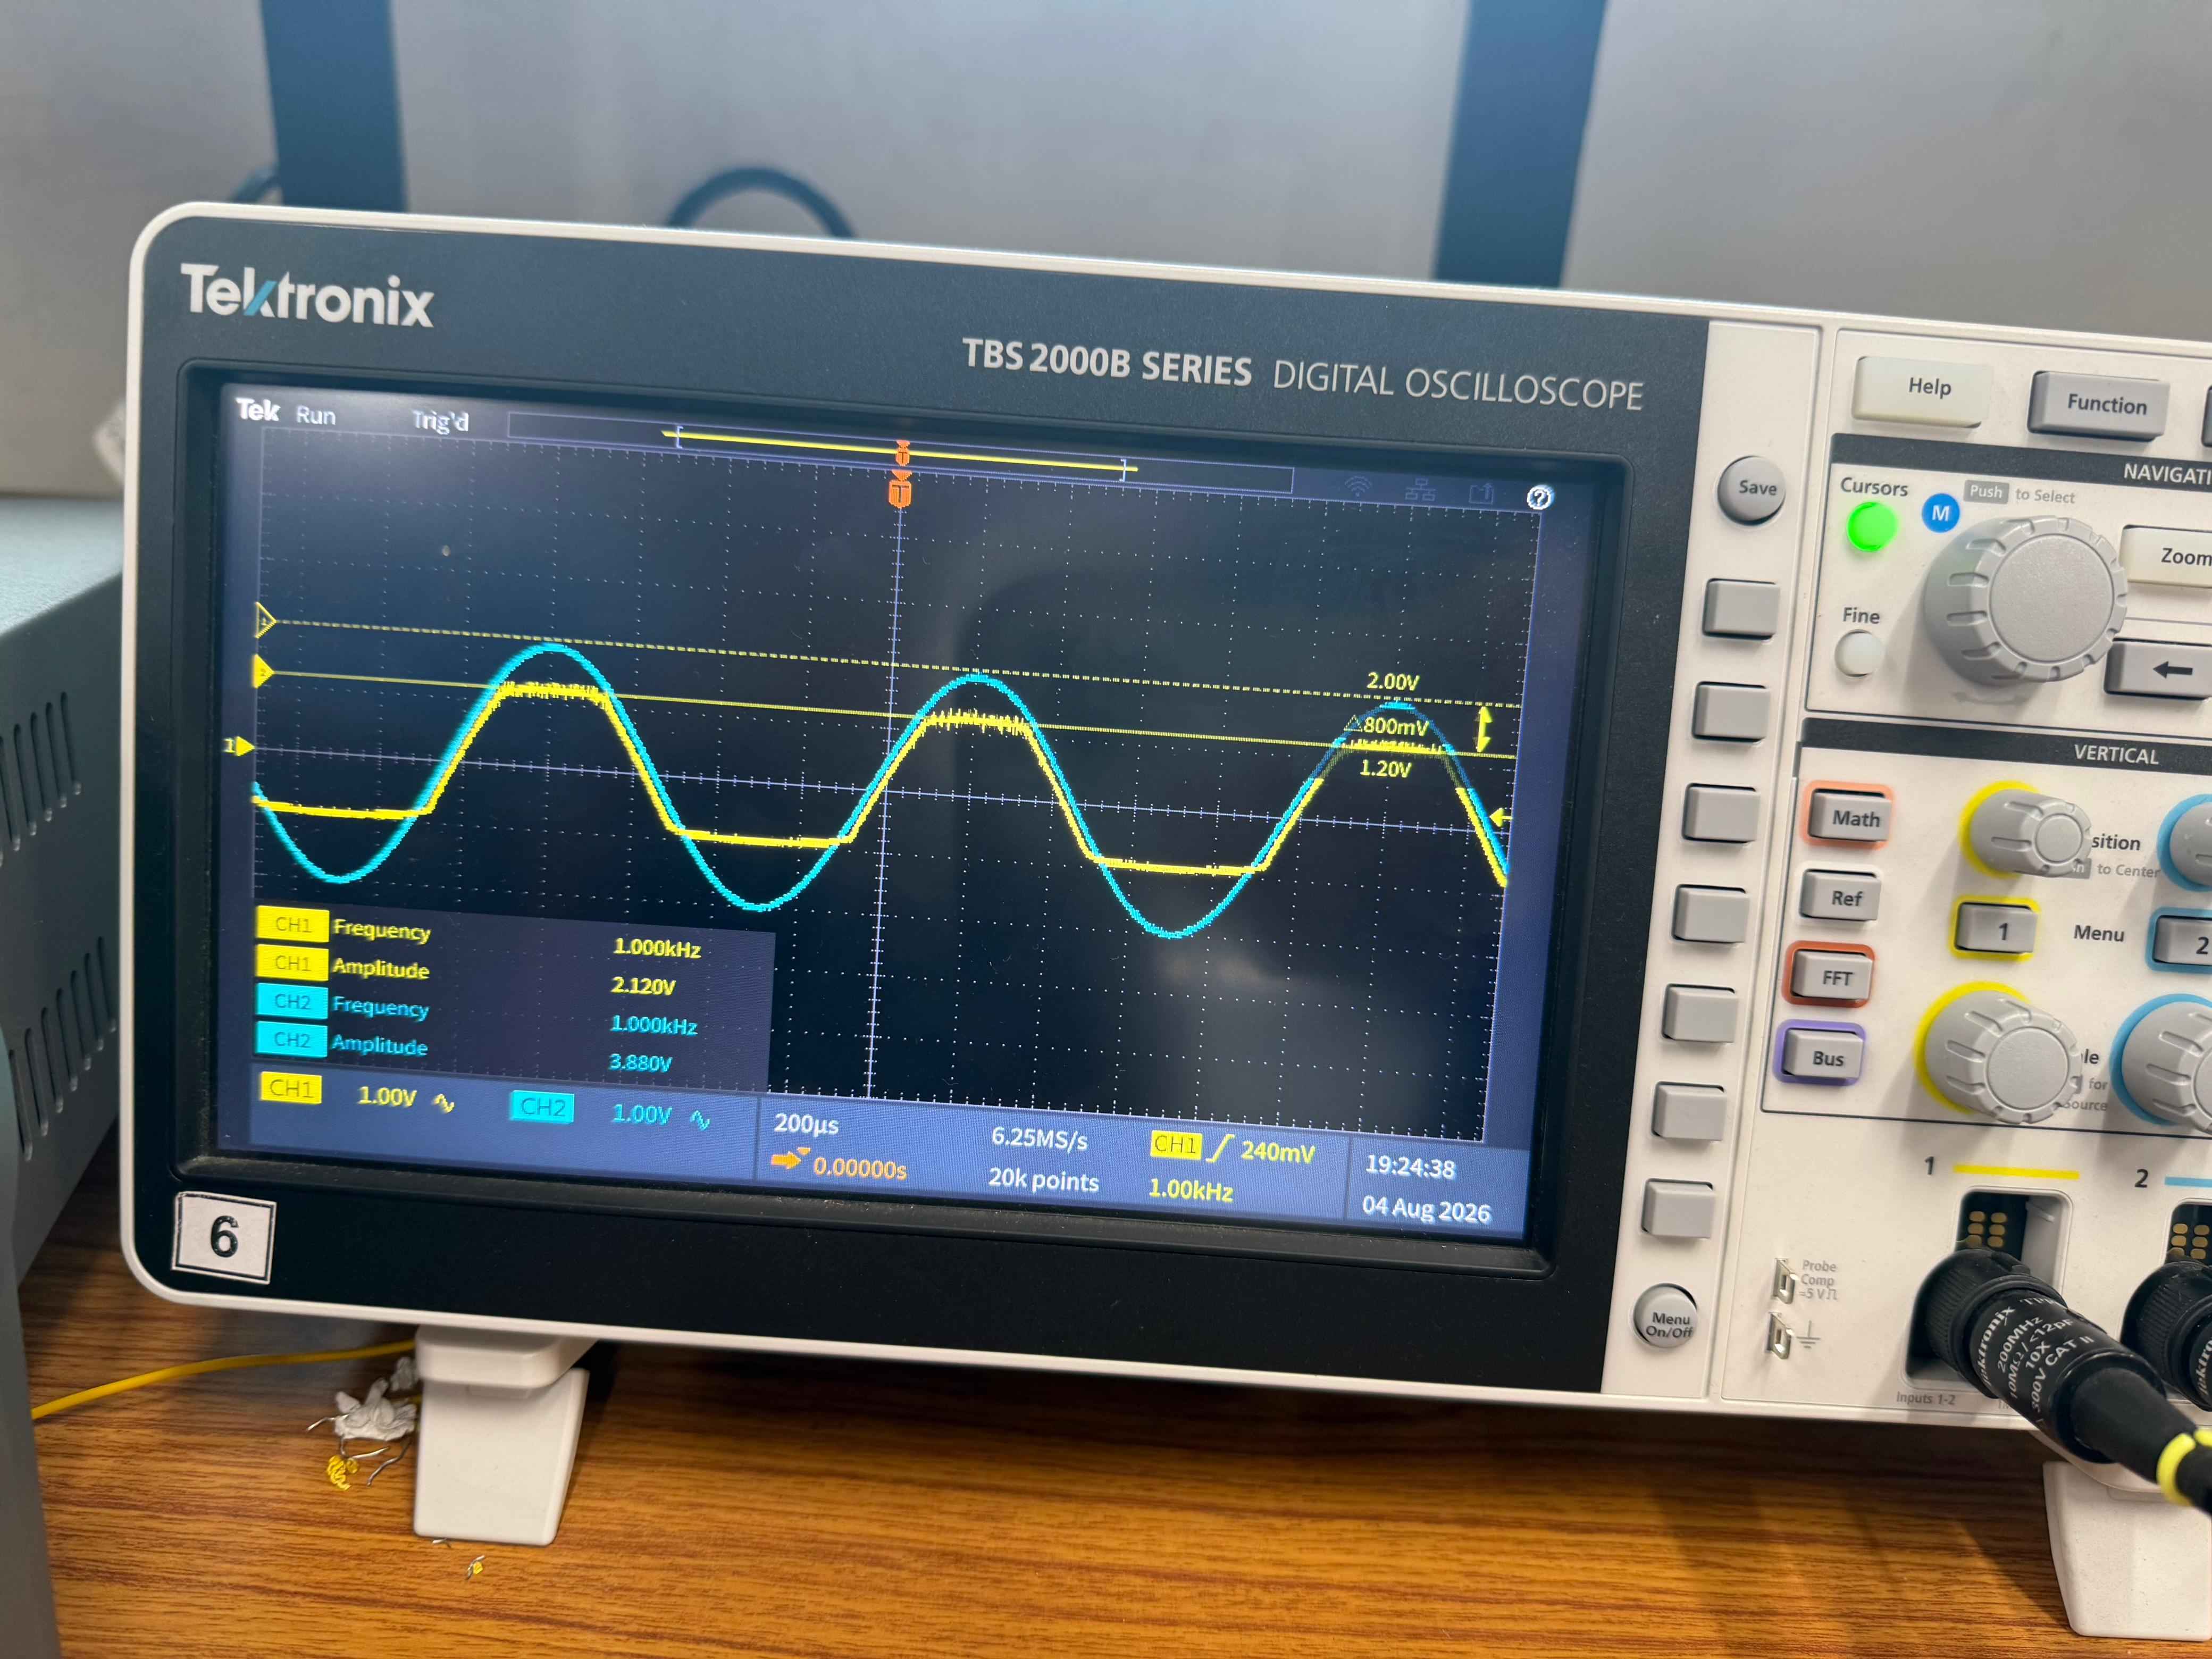
\includegraphics[width=\textwidth]{../BIASED_CLIPPER/dso_biased_clip_1.jpeg}
        \caption{DSO Trace}
    \end{subfigure}
    \caption{Biased Clipper Circuit, Simulation, and Measured DSO Waveform (Clipped at $+1.20\text{ V}$ \& $-0.92\text{ V}$).}
    \label{fig:biased_clipper}
\end{figure}

\subsection{Clipper Experimental Observation Summary}
\begin{table}[H]
\centering
\caption{Diode Clipper Circuits Observation Table ($R_L = 100\text{ k}\Omega$)}
\begin{tabular}{l c c c l}
\toprule
\textbf{Circuit} & \textbf{Input $V_{pp}$ (V)} & \textbf{Theoretical Clip Level} & \textbf{Measured Clip Level} & \textbf{Inference} \\
\midrule
Positive Clipper & 4.0 & $+1.0\text{ V} + V_\gamma \approx +1.65\text{ V}$ & Clip at $+1.60\text{ V}$ & Upper peak clipped cleanly above $V_{ref}+V_\gamma$. \\
Negative Clipper & 4.0 & $-1.0\text{ V} - V_\gamma \approx -1.65\text{ V}$ & Clip at $-1.68\text{ V}$ & Lower peak clipped cleanly below $-V_{ref}-V_\gamma$. \\
Biased Clipper   & 4.0 & $+1.65\text{ V}$ \& $-1.65\text{ V}$ & $+1.20\text{ V}$ \& $-0.92\text{ V}$ & Dual-level clipping limits peak-to-peak swing. \\
\bottomrule
\end{tabular}
\end{table}

\newpage
\section{Part D: Diode Clamper Circuits}

\subsection{Theoretical Background}
Clampers shift an AC waveform vertically by clamping one peak to a fixed DC level without distorting the peak-to-peak amplitude. A load resistor $R_L = 100\text{ k}\Omega$ was connected across the output node to ensure smooth readings and proper discharge behavior of capacitor $C = 0.1\text{ }\mu\text{F}$.

\subsection{Circuit Diagrams, Simulations \& Hardware DSO Waveforms}

\subsubsection{Positive Clamper}
The positive clamper shifts the waveform upward such that the negative peak is clamped near $-V_\gamma = -0.52\text{ V}$.
\begin{figure}[H]
    \centering
    \begin{subfigure}[b]{0.32\textwidth}
        \centering
        
\includegraphics[width=\textwidth]{../POSITIVE_CLAMPER/circuit.png}
        \caption{Circuit Schematic}
    \end{subfigure}
    \hfill
    \begin{subfigure}[b]{0.32\textwidth}
        \centering
        
\includegraphics[width=\textwidth]{../POSITIVE_CLAMPER/sim.png}
        \caption{LTspice Simulation}
    \end{subfigure}
    \hfill
    \begin{subfigure}[b]{0.32\textwidth}
        \centering
        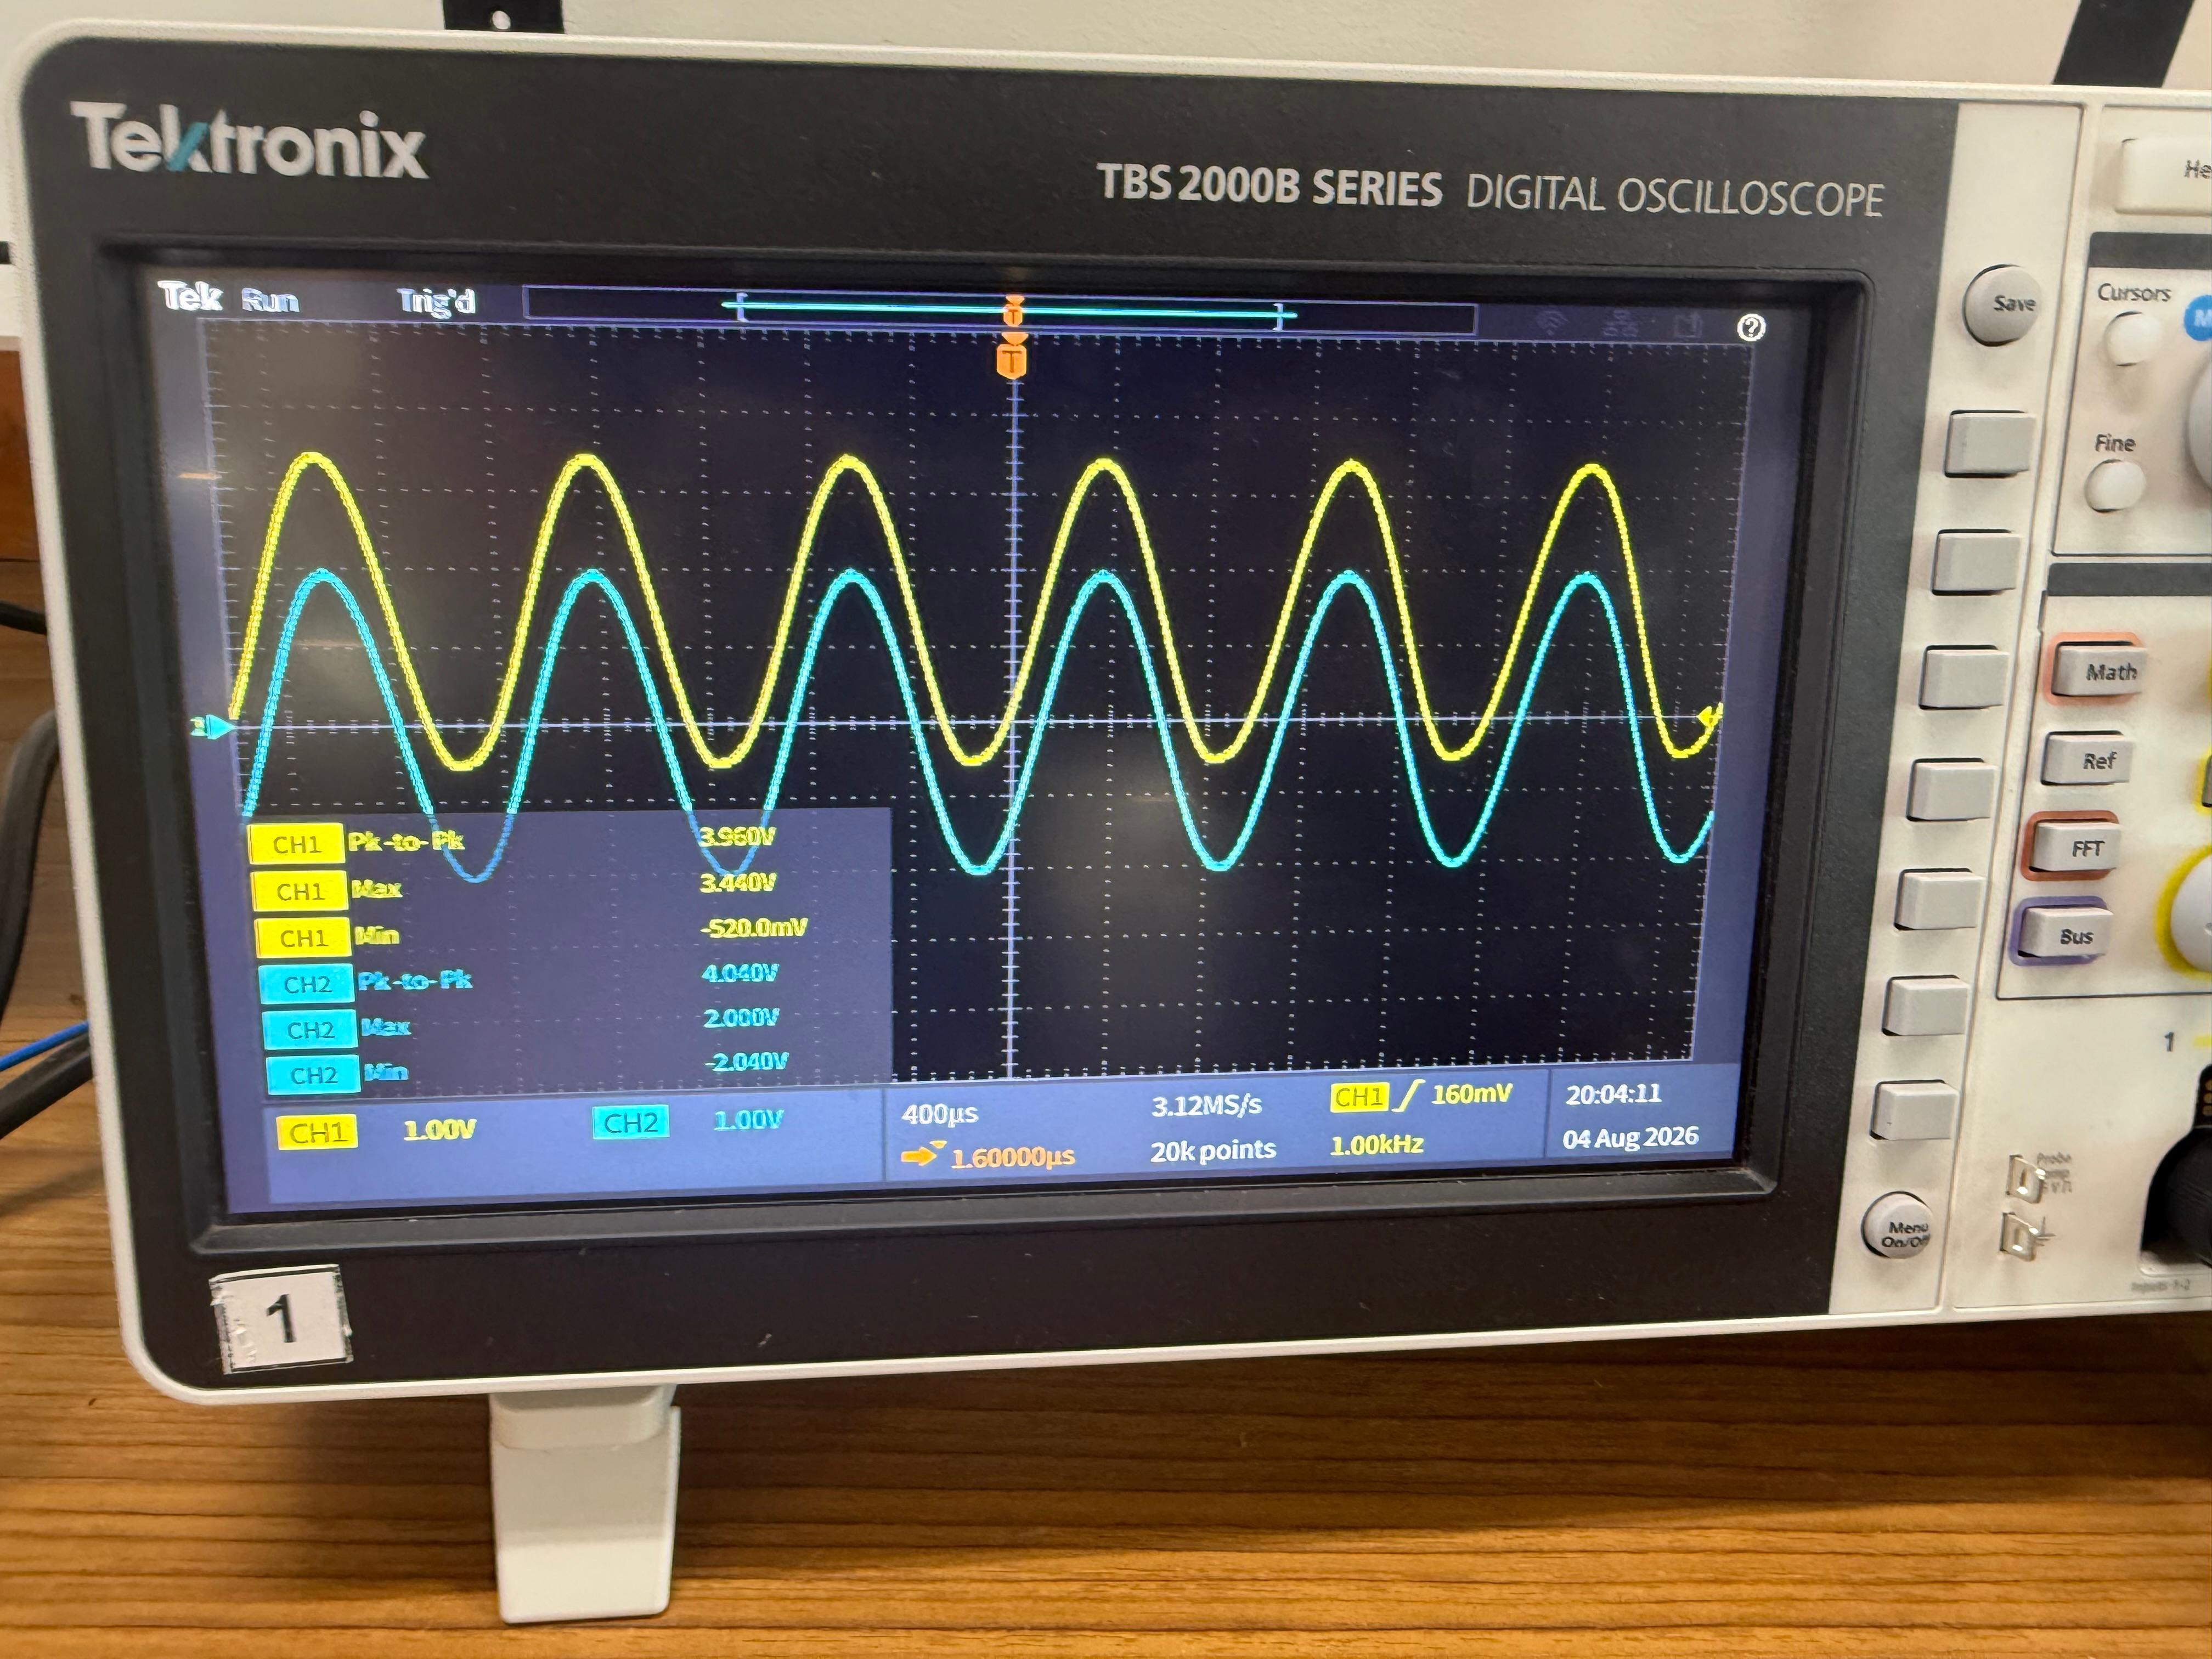
\includegraphics[width=\textwidth]{../POSITIVE_CLAMPER/dso_pos_clamp.jpeg}
        \caption{DSO Trace}
    \end{subfigure}
    \caption{Positive Clamper Circuit, Simulation, and Measured DSO Waveform (Min level at $-0.52\text{ V}$).}
    \label{fig:pos_clamper}
\end{figure}

\subsubsection{Negative Clamper}
The negative clamper shifts the waveform downward such that the positive peak is clamped near $+V_\gamma = +0.56\text{ V}$.
\begin{figure}[H]
    \centering
    \begin{subfigure}[b]{0.32\textwidth}
        \centering
        
\includegraphics[width=\textwidth]{../NEGATIVE_CLAMPER/circuit.png}
        \caption{Circuit Schematic}
    \end{subfigure}
    \hfill
    \begin{subfigure}[b]{0.32\textwidth}
        \centering
        
\includegraphics[width=\textwidth]{../NEGATIVE_CLAMPER/sim.png}
        \caption{LTspice Simulation}
    \end{subfigure}
    \hfill
    \begin{subfigure}[b]{0.32\textwidth}
        \centering
        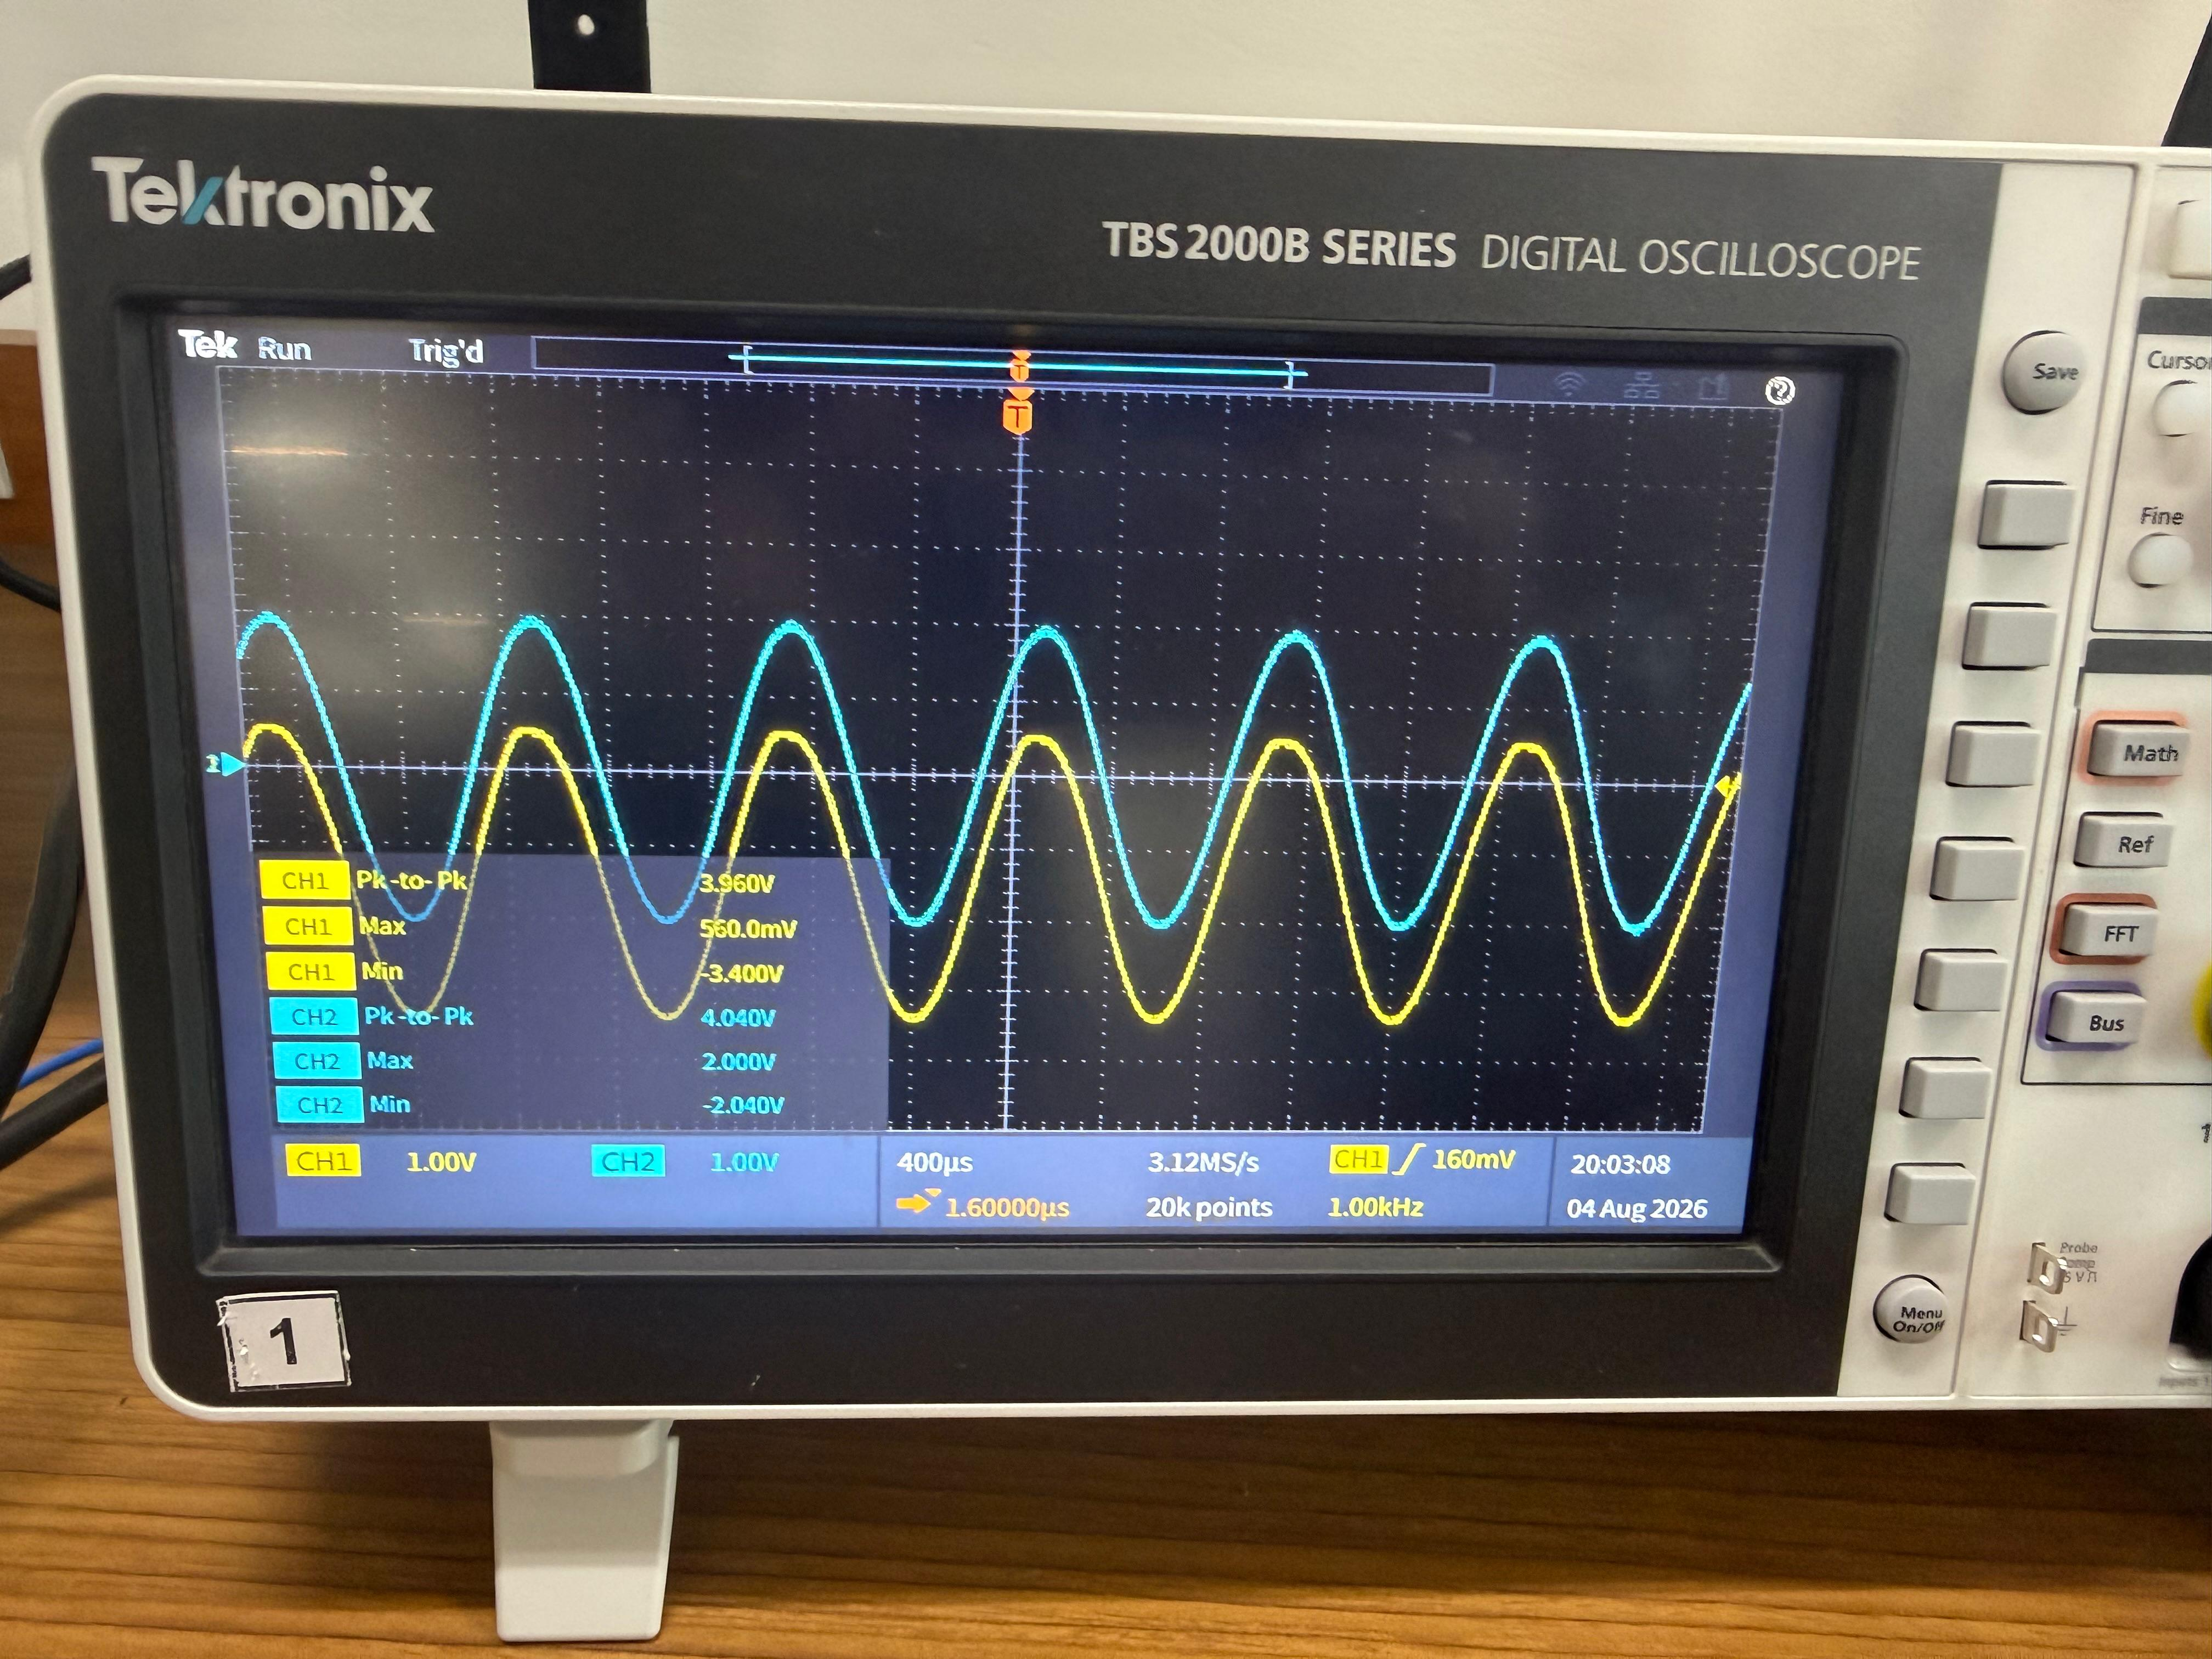
\includegraphics[width=\textwidth]{../NEGATIVE_CLAMPER/dso_neg_clamp.jpeg}
        \caption{DSO Trace}
    \end{subfigure}
    \caption{Negative Clamper Circuit, Simulation, and Measured DSO Waveform (Max level at $+0.56\text{ V}$).}
    \label{fig:neg_clamper}
\end{figure}

\subsection{Clamper Experimental Observation Summary}
\begin{table}[H]
\centering
\caption{Diode Clamper Circuits Observation Table ($R_L = 100\text{ k}\Omega$)}
\begin{tabular}{l c c c l}
\toprule
\textbf{Circuit} & \textbf{Input $V_{pp}$ (V)} & \textbf{Theoretical Shift} & \textbf{Measured Clamped Level} & \textbf{Inference} \\
\midrule
Positive Clamper & 4.0 & Shift up by $+V_p - V_\gamma \approx +1.30\text{ V}$ & Min level at $-0.52\text{ V}$ & Upward DC shift; min level clamped at $-V_\gamma$. \\
Negative Clamper & 4.0 & Shift down by $-V_p + V_\gamma \approx -1.30\text{ V}$ & Max level at $+0.56\text{ V}$ & Downward DC shift; max level clamped at $+V_\gamma$. \\
\bottomrule
\end{tabular}
\end{table}

\section{Discussion \& Overall Inferences}
\begin{enumerate}
    \item \textbf{PN Diode Non-linearity \& Conduction:} Forward bias readings demonstrate exponential growth after overcoming cut-in barrier voltage \textbf{$V_\gamma \approx 0.60\text{ V}$}. Semi-log plots confirm Shockley's relation with linear slope in forward conduction. Static resistance decreases from \textbf{$R_{DC} = 283.78\text{ }\Omega$} at $2.22\text{ mA}$ to \textbf{$R_{DC} = 36.50\text{ }\Omega$} at $20.0\text{ mA}$, while dynamic resistance settles at \textbf{$r_d = 3.07\text{ }\Omega$}.
    \item \textbf{Zener Breakdown Regulation:} In reverse bias, breakdown occurs sharply at \textbf{$V_Z \approx 5.00\text{--}5.25\text{ V}$}. The low dynamic Zener resistance \textbf{$R_Z = 14.53\text{ }\Omega$} confirms excellent voltage regulation stability under varying reverse currents.
    \item \textbf{Clipper Behavior:} Incorporating a \textbf{$100\text{ k}\Omega$ load resistor} prevented signal attenuation. Clipping thresholds closely match $V_{ref} \pm V_\gamma$ (\textbf{$+1.60\text{ V}$} for positive, \textbf{$-1.68\text{ V}$} for negative, and \textbf{$+1.20\text{ V} / -0.92\text{ V}$} for biased clipper).
    \item \textbf{Clamper DC Restoration:} Positive and negative clampers successfully restore the DC level, shifting the minimum peak to \textbf{$-0.52\text{ V}$} and maximum peak to \textbf{$+0.56\text{ V}$} respectively without altering the peak-to-peak amplitude.
\end{enumerate}

\end{document}
